\documentclass[smallcondensed]{svjour3}

\usepackage[T1]{fontenc}
\usepackage[utf8]{inputenc}
\usepackage[authoryear]{natbib}
\usepackage{graphicx}
\usepackage{amssymb}
\usepackage{color}
\usepackage{lscape}
\usepackage{tabularx}
\usepackage{tabulary}
\newtheorem{Hypothesis}{Hypothesis}
\setcitestyle{aysep={}}

\begin{document}
\title{Need, Equity, and Accountability}
\subtitle{Evidence on Third-Party Distribution Decisions from a Vignette Study}
\author{Alexander Max Bauer \and Frauke Meyer \and Jan Romann \and Mark Siebel \and Stefan Traub}
\institute{Alexander Max Bauer \at Corresponding Author, University of Oldenburg, Department of Philosophy, Ammerl\"ander Heerstra{\ss}e 114--118, 26129 Oldenburg, Germany, \email{alexander.max.bauer@uol.de}, ORCID: 0000-0003-0923-6864 \and Frauke Meyer \at Forschungszentrum J\"ulich GmbH, Institute of Energy and Climate Research---Systems Analysis and Technology Evaluation (IEK--STE), 52425 J\"ulich, Germany \and Jan Romann \at University of Bremen, SOCIUM Research Center on Inequality and Social Policy, 28359 Bremen, Germany \and Mark Siebel \at University of Oldenburg, Department of Philosophy, 26129 Oldenburg, Germany \and Stefan Traub \at Helmut-Schmidt-University Hamburg, Department of Economics, 22043 Hamburg, Germany}
\thanks{The authors are members of the research group ``Need-Based Justice and Distributive Procedures'' (FOR 2104) funded by the German Research Foundation (DFG Grants SI 1731/2-2, TR 458/6-2). We are grateful for the support and input throughout all project phases from participants of the FOR 2104 meetings. We thank Densua Mumford for proofreading the manuscript and participants at the 1st European Experimental Philosophy Conference for comments. We also thank three anonymous referees for their helpful and constructive comments.}
\maketitle
%
\noindent\textbf{Abstract:} We report the results of a vignette study with an online sample of the German adult population in which we analyze the interplay between need, equity, and accountability in third-party distribution decisions. We asked participants to divide firewood between two hypothetical persons who either differ in their need for heat or in their productivity in terms of their ability to chop wood. The study systematically varies the persons' accountability for their neediness as well as for their productivity. We find that participants distribute significantly fewer logs of wood to persons who are held accountable for their disadvantage. Independently of being held accountable or not, the needier person is partially compensated with a share of logs that exceeds her contribution, while the person who contributes less is given a share of logs smaller than her need share. Moreover, there is a domain effect in terms of participants being more sensitive to lower contributions than to greater need.\\[0.5ex]
%
\noindent\textbf{Keywords:} Need, Equity, Accountability, Justice, Vignette Study\\
\textbf{JEL Classification:} I39, D63, D31
%
\section{Introduction}\label{sec:introduction}
%
This paper contributes to the growing empirical social choice literature which was initiated by the investigations of participants' individual and group distribution choices by \citet{yaari_dividing_1984} as well as \citet{frohlich_choices_1987} (for overviews see, for example, \citealt{konow_which_2003}, \citealt{traub_friedman_2005}, \citealt{konow_is_2009}, as well as \citealt{gaertner_empirical_2012}). This literature shows that participants' distribution preferences are pluralistic and context-dependent \citep{konow_economics_2016}. Distribution preferences are pluralistic if they consist of multiple fairness criteria. They are context-dependent if the weight that is given to each criterion depends on institutional factors and personal traits. Apart from the two most important criteria, equality and equity, need has also been identified as relevant in pluralistic justice theories (\citealt{konow_fair_2001, konow_which_2003}, \citealt{nicklisch_need_2020}). Moreover, several studies (see, for example, \citealt{konow_fair_2001} and \citealt{schwettmann_trading_2009}) have found that people's support for need-based fairness is balanced against accountability.\par
%
However, apart from these stylized facts, not much is known about the quantitative relationship between distribution principles like need and equity, on the one hand, and moderating factors like accountability, on the other hand. In this paper, we will contribute to filling this gap by reporting the results of a vignette study with an online sample of the German adult population in which we analyze the interplay between need, equity, and accountability in third-party distribution decisions.\par
%
Following \citep{miller_principles_1999}, we define need as the amount of some good that a member of society requires in order to \textit{avoid harm}. Equity is understood as a variant of Aristotle's proportionality principle, which holds that output should be allocated in proportion to the participant's \textit{contribution} in terms of her productive work effort \citep{konow_positive_1996}. The accountability principle \citep{konow_fair_2001} is implemented both as \textit{responsibility for contribution to output} and as \textit{responsibility for need}.\par
%
Participants, who were recruited by an online platform, were asked to divide firewood needed for heating in winter between two hypothetical persons who differed in their need for heat and their productivity in terms of their ability to chop wood (and thus to contribute to the total stock of firewood available). As a novel feature, the study systematically varied the hypothetical persons' accountability for their neediness as well as for their lower productivity in two separate scenarios.\par
%
Our main results are as follows. On average, participants distributed significantly fewer logs of wood to persons who were held accountable for their disadvantage in terms of exhibiting greater need or lower productivity. Independently of being held accountable or not, the needier person was always partially compensated for her disadvantage with a share of logs that exceeded her contribution, while the person who contributed less was given a share of logs smaller than her need share.\par
%
When accountability was low, participants did not differentiate between the source of a person's disadvantage when compensating her with additional logs, that is, greater need and lower productivity were processed symmetrically. In contrast to this, high accountability gave rise to an asymmetry where a disadvantaged person's compensation was significantly \textit{smaller} when her disadvantage was due to lower productivity instead of greater need.\par
%
We explain this asymmetry by reference points and loss aversion \citep{tversky_loss_1991}, that is, a gain-loss domain effect. If participants perceive the equal-split distribution of logs as a natural reference point \citep{yaari_dividing_1984}, loss averse participants might recode the compensation for a self-inflicted disadvantage in terms of a contribution falling \textit{below} half of the total logs as the reduction of a loss (negative domain) and the compensation for a self-inflicted disadvantage in terms of need \textit{exceeding} half of the total logs as a gain (positive domain). Hence, due to loss aversion, the former case requires a smaller compensation to establish a just distribution of logs.\par
%
Increasing inequality (in terms of different need or productivity) among the two persons left the relative weight put to need and equity unchanged. One case where the disadvantaged person had a deficit of logs and the other person had a surplus made an exception. Here, some participants applied the ``net split'' principle where both persons received the absolute number of logs they needed plus (or minus) half of the oversupply (or undersupply) of logs.\par
%
The analysis of individual choices confirmed that participants were less generous towards the person who was accountable for her own disadvantage. It also showed that the negative impact of accountability was both due to a larger share of participants choosing not to compensate the disadvantaged person at all (extensive margin) and a diminished willingness to compensate her partially (intensive margin). Some participants applied complex distribution principles like the ``net split'' which cannot be formally represented by a simple convex combination of need, equity, and equality.\par
%
Our result concerning the impact of accountability on distribution choices is in line with the vast majority of the empirical and experimental social choice literature which will be reviewed in Section \ref{sec:literature}. For example, \citet{schwettmann_competing_2012}, who also used a ``heating-in-winter'' scenario, found that when the disadvantage of the worse-off individuals was caused by their ``careless behaviour'' (p.~368), participants chose significantly less often the options that lifted the disadvantaged individual to the poverty line.\par
%
\citet{schwettmann_competing_2012} and related studies usually present participants with an exogenously given choice set of distributions that correspond to specific distribution principles such as egalitarianism, Rawls' maximin principle, or truncated utilitarianism. In our study, we take a different approach by letting participants freely choose how many logs of wood they want to distribute to the persons who differ in their need and productivity. Eliminating the fixed choice set avoids a possible drawback of the expert approach, namely, researcher's bias \citep{ahlert_thresholds_2012}, and gives room for behavior more in line with participants' rather pluralistic opinions about distributive justice.\par
%
\citet{gaertner_empirical_2012} comprehensively address methodological issues regarding empirical social choice. They also dwell on the pros and cons of (incentivized) lab and (non-incentivized) survey experiments. Empirical research on justice is useful for several reasons. For example, our study, which uses a stratified sample of the German adult population, shows that justice attitudes are linked to personal characteristics such as income; we discover unusual distribution principles like the ``net split''; and we contribute data to the development of ``empirically informed'' pluralistic and context-dependent theories of justice \citep{konow_economics_2016}. While game-theoretic experiments make predictions about actual behavior, which is to some extent driven by self-interest, \citet{gaertner_empirical_2012} underline that the aim of empirical social choice is to derive information about people's norms. Vignette studies ``provide a contextual richness that is better suited'' than incentivized experiments to study fairness judgments embedded in real social institutions \citep[p. 109]{konow_is_2009}.\par
%
The paper is organized as follows. Section \ref{sec:literature} reviews the theoretical background of this study and introduces previous empirical research on the matter. In Section \ref{sec:design}, we outline the research design, before presenting the data analysis and results in Section \ref{sec:results}. Section \ref{sec:conclusion} concludes the paper.\par
%
\section{Literature Review}\label{sec:literature}
%
Needs play an important role in political theory (\citealt{doyal_theory_1984},\citealt{weale_political_1984}, \citealt{nussbaum_human_1992}, \citealt{dean_translation_2013}), as a policy goal (\citealt{esping-andersen_three_1990}, \citealt{boarini_measures_2006}), and are deeply linked with conceptions of the welfare state (\citealt{dean_welfare_2002}, \citealt{plant_political_2009}). Because of their fundamental nature---they refer to the basic conditions for human existence---needs have also been proposed by many as the principal normative grounding for human rights (see, for example, \citealt{brock_needs_2005}, \citealt{gasper_needs_2005}, and \citealt{renzo_human_2015}). As a distributional criterion, need also features prominently in positive justice research (see, for example, \citealt{frohlich_choosing_1990}, \citealt{scott_just_2001}, \citealt{konow_which_2003}, \citealt{michelbach_doing_2003}, \citealt{scott_whats_2009}, as well as \citealt{sabbagh_sociology_2016}), suggesting that voters, too, care about needs.\par
%
A need can be understood as an amount of some good that a member of society requires in order to \textit{avoid harm} (see \citealt{miller_principles_1999}, for an overview on philosophical approaches to need-based justice, see \citealt{siebel_need-based_2020} as well as \citealt{miller_needs-based_2020}). Some needs are biological (for example, the amount of calories a person should consume every day), while many others are social in nature (for example, the amount of money necessary to participate in social life). What separates needs from mere wants is, among other things, that the former are based on a socially shared understanding \citep{miller_principles_1999}. That is, for someone's want to become a need, others must \textit{acknowledge} that it is necessary for her in order not to be harmed. As an inter-subjectively acknowledged threshold, needs provide a fundamentally different basis of social justice than other criteria, such as equality, equity, and the Rawlsian maximin principle.\par
%
Equity is understood here in terms of Aristotle's proportionality principle, which relates a person's entitlement to her \textit{contribution} (\citealt{aristotle_nicomachean_2009}, \citealt{young_equity_1994}). Hence, in equity theory (\citealt{homans_social_1958}, \citealt{adams_inequity_1965}), this principle is often called the ``contribution principle'' (compare \citealt{diederich_identifying_2020}).\par
%
Our understanding of accountability is based on Konow's ``principle of accountability''. He states that this principle ``calls for allocations to be in proportion to volitional contributions'' \citep[p. 138]{konow_fair_2001} and that ``individuals are only held accountable for factors they may reasonably control'' \citep[p.~142]{konow_fair_2001}. Hence, the accountability principle differentiates between \textit{actual} and \textit{controllable} contributions.\par
%
In the context of distributive justice, one might also think of luck egalitarianism, which argues that someone being worse-off than others can only be justified if she is not accountable for her situation. The effects of ``brute luck'', therefore, should be compensated, while those resulting from ``option luck'' do not qualify for compensation (see, for example, \citealt{dworkin_equality_1981}, \citealt{temkin_inequality_1993}, \citealt{knight_luck_2009}, \citealt{cohen_currency_2011}, and \citealt{tan_justice_2012}; an experimental investigation on attitudes towards compensation and risk-taking can be found in \citealt{cappelen_just_2013}). Theoretical considerations in economics are also relevant. For example, \citet{cappelen_responsibility_2005, cappelen_responsibility_2006}, \citet{cappelen_relocating_2006}, as well as \citet{cappelen_disability_2010} investigated the possible relevance of accountability for liberal egalitarian theories of justice.\par
%
From an empirical point of view, \cite{konow_is_2009} highlighted that many empirical and experimental studies have found preferences for unequal distributions, giving room for principles other than equality (for some examples that also include the principle of need, see \citealt{deutsch_equity_1975}, \citealt{leventhal_distribution_1976}, \citealt{lerner_justice_1977}, \citealt{lamm_norms_1980}, \citealt{deutsch_distributive_1985}, \citealt{scott_just_2001}, and \citealt{cappelen_rich_2008}).\par
%
Concerning need, participants have been found to prefer distributions that grant a minimum income to everyone. For example, \citet{ahlert_thresholds_2012} have reported great support for the need principle in terms of ``truncated utilitarianism'' or a ``truncated split'' in a modified dictator game. \citet{frohlich_choosing_1992} have demonstrated that maximizing the average income with a floor constraint is the overwhelmingly preferred distribution principle by groups \citep[also see][]{frohlich_choices_1987}.\par
%
Concerning accountability, \citet{weiner_sin_1993} has found that being accountable leads to greater reward or punishment. \citet{weiner_attributional_1970} have also demonstrated that lack of effort is punished more severely than lack of ability. \citet{mellers_ants_1993, skitka_providing_1993} have shown that personal ideological orientation influences whether accountability has an impact on distribution decisions. Conservatives are in favor of withholding public assistance to people who are accountable for their predicament while liberals tend to help everyone. \citet{konow_positive_1996} has found support for the assumption that persons are only held accountable for variables they can control (for example a person's work effort).\par
%
Moreover, there are some studies that explore need and accountability in combination. \citet{lamm_norms_1980} investigated the influence of social proximity and accountability, calling it ``the perceived causal locus of the needs'' (p. 426). However, they did not find a significant influence of accountability on distribution choices. \citet{gaertner_equity_2007} used questionnaire-experimental studies to assess participants' justice evaluations for scenarios that involved trade-offs between basic needs on the one hand and efficiency or accountability on the other hand. Incorporating a more efficient choice alternative often led to decisions against the needy person. Introducing personal accountability (in terms of having an innate or acquired handicap) had, if at all, a rather weak impact on justice evaluations. Using a charity game, \citet{buitrago_relation_2009} explored whether it makes a difference if the causes of neediness were known or not, including cases in which neediness was self-inflicted by low effort. They did not find a significant effect, concluding that ``help attitudes may result from idiosyncratic preferences, which are unaffected by the causes of neediness'' (p. 83).\par
%
In contrast to this, \citet{konow_fair_2001} found that telephone and questionnaire survey participants' support for need-based justice was balanced against both accountability and efficiency. \citet{schwettmann_competing_2012}, using a questionnaire study, presented participants with distribution problems that required them to distribute a resource between two groups, providing them with information on benefit, need, efficiency, and accountability. He found strong support for need-oriented distribution choices that were not influenced by concerns for efficiency. Accountability, though, had a significant impact on distribution decisions. When a group was accountable for a shortage of supplies, fewer participants decided to lift its members up to the need threshold. Furthermore, \citet{cappelen_needs_2013} has found evidence for the influence of need (represented by subjects from low-income countries) and accountability (represented by ``entitlement'' through real-effort tasks) in a dictator game.\par
%
\citet{skitka_allocating_1992} have investigated the influence of the causes of neediness on subjects' readiness to help others. They concluded that subjects ``are least likely to help victims whose need is attributed to internal-controllable causes---such as carelessness, laziness, greed, and self indulgence'' (pp. 496f.). This conclusion is supported by other studies, which all find that performance and accountability have an influence on the support for need as a distribution criterion (see \citealt{wagstaff_equity_1994}, \citealt{farwell_self-perception_1996}, as well as \citealt{scott_whats_2009}).\par
%
A considerable literature deals with medical interventions that can obviously be considered as situations of (basic) need satisfaction. For example, \citet{ubel_allocation_2001} investigated the influence of accountability on hypothetical decisions for the allocation of transplant livers (also see \citealt{neuberger_assessing_1998}). Those who were accountable for their illness received the transplant less often. \citet{diederich_zur_2010} have confirmed the relevance of accountability for prioritization in health care using a mixed-methods design (also see \citealt{diederich_does_2014}). Similar results have been obtained by \citet{betancourt_attribution-empathy_1990}, \citet{karasawa_effects_1991}, \citet{murphy-berman_factors_1984}, \citet{turner_depalma_perceived_1999}, as well as \citet{yamauchi_attribution-emotion_1999}. \citet{annas_prostitute_1985} and \citet{stanton_cost_1999} have shown the relevance of accountability for the allocation of scarce life-saving technology. Finally, \citet{fowler_measuring_1994} have shown that clinical services directed at patients that can be held accountable for their illness were considered a lower priority.\par
%
In summary, apart from a small number of exceptions, the literature finds---in a wide range of different scenarios---a significant negative impact of a person's accountability for her neediness on other persons' willingness to distribute resources to her. This paper contributes to this literature by reporting the results of a novel vignette study with an online sample of the German adult population that analyzes the interplay between need, equity, and accountability in third-party distribution decisions.\par
%
In the following section, we introduce the design of our vignette study. As noted by \citet{konow_which_2003}, vignette studies provide a flexible and easily controllable way to present relevant contextual information to participants. In particular, the empirical social choice literature, pioneered by \citet{yaari_dividing_1984}, relies on such designs to study preferences for distributions in hypothetical scenarios (overviews are given by \citealt{schokkaert_m_1999}, \citealt{schwettmann_trading_2009}, as well as \citealt{gaertner_empirical_2012}). As suggested by \cite{konow_which_2003,konow_blind_2005}, subjects acted as impartial decision-makers in order to avoid self-serving bias. Like \citet{schwettmann_competing_2012}, we used heating in winter as a background story. The accountability framing followed \citet{diederich_zur_2010}, who also used smoking and hereditary factors as causes for a disease, as well as \citet{skitka_allocating_1992}, who also named the disregard of a doctor's warning and a gene defect as causes for low and high accountability.\par
%
However, most of the above mentioned experimental social choice studies (for example, \citealt{gaertner_equity_2007}, \citealt{schwettmann_competing_2012}, and \citealt{ahlert_thresholds_2012}) are based on sets of predefined choice alternatives in terms of distributions of resources among two or more persons that correspond to certain \textit{normative} distribution principles (such as egalitarianism, Rawls' maximin criterion, and truncated utilitarianism). That is, in these settings, subjects or groups make choices between standards of behavior that were devised by experts. Like in a beauty contest, the standard of behavior that is met with the greatest approval from subjects is declared the winner.\par
%
A distinct advantage of this expert driven approach is its ability to provide direct tests of certain axioms and normative theories of distributive justice (see \citealt{frohlich_choices_1987} for a prototypical experiment; see \citealt{bauer_philosophie_2019, bauer_empirical_2020} for general considerations on the interplay of empirical research and normative theory). A drawback of this approach is that such preselections may involve researcher's bias \citep{ahlert_thresholds_2012}. Related to the previous argument, people's opinions about distributive justice frequently are in conflict with these traditional norms and assumptions (see \citealt{schokkaert_m_1999}; also see \citealt{amiel_thinking_1999} as well as \citealt{traub_friedman_2005}). Moreover, as noted by \citet{ahlert_thresholds_2012}, rankings of \textit{monistic} distribution principles according to their approval by subjects in choice experiments do not adequately reflect the fact that ``pluralism of distribution principles is the predominant outcome of many empirical investigations'' (p.~980; also see \citealt{konow_which_2003}).\par
%
Consequently, although this study has been heavily inspired by the aforementioned literature, we took a different path by letting participants freely choose how much of a given resource they want to distribute among two persons who differ in their need, productivity, and accountability. This procedure is similar to Question 3 in \citep{konow_is_2009}. A related approach, though in a modified dictator-game setting, was taken by \citet{andreoni_giving_2002} as well as \citet{fisman_individual_2007}, who let subjects divide fixed amounts of tokens between themselves and another subject with varying prices for payoffs. Hence, whether or not these endogenously determined distributions meet certain distribution principles is an outcome of the study. The main goal of this paper is to quantitatively measure the impact of giving information on accountability on participants' distribution decisions while systematically varying recipients' need and productivity.\par
%
\section{Study Design}\label{sec:design}
%
In Subsection \ref{sec:vignettes}, we first describe the vignette-based study design. In Subsection \ref{sec:procedure}, we then describes the procedure of the study. After that, in Subsection \ref{sec:hypotheses}, we formulate working hypotheses about the impact of different accountability framings and scenarios on participants' distribution choices.\par
%
\subsection{The Vignettes}\label{sec:vignettes}
%
In the vignettes, we asked participants to imagine two persons, denoted ``Person A'' and ``Person B'', who do not know each other (for the instructions and the exact wording of the vignette, see Appendix \ref{sec:app_instructions}; we used a set of common German surnames to identify the protagonists). Participants were told that these two persons heat their homes exclusively with firewood and that both have enough logs in stock to survive the upcoming winter. Nonetheless, they need additional firewood so that they will not feel cold. With this in mind, the community allows them to chop wood in the community forest for a certain period of time. Both A and B have little money and, therefore, they have no other means of getting firewood or any other heating material.\par
%
In accordance with our definition of need as the amount of some good that a member of society requires in order to avoid harm, the vignettes described the consequences of unfulfilled need (``If they get less than they need, it will get unreasonably cold in their huts. The less firewood they get, the colder their huts will be.''). The participants' task was to distribute an exogenously given number of logs among A and B. In order to justify unequal distributions of logs, we introduced heterogeneity between A and B with respect to their \textit{need} for logs, or their \textit{productivity} in terms of the number of logs contributed, and their \textit{accountability} for their situation.\par
%
Participants' distribution choices therefore reveal how far need is \textit{acknowledged}, and whether and how the acknowledgment of need is affected by the two persons' heterogeneity. Note that we intentionally described the consequences of unfulfilled need as mildly harmful (``[\ldots] it will become unreasonably cold in their huts.'') and not as life threatening in order to leave participants more scope for judgment. We also allowed for over-fulfillment of need (``The persons can use more firewood than they need to heat their huts up to pleasant temperatures or store it for subsequent winters.'') in order to study how participants handle mixed situations (where one person has unfulfilled need and the other has fulfilled need) and situations of ``oversupply'' (where both persons have different fulfilled needs).\par
%
In the following, we call the framing of the vignette with respect to need and productivity \textit{scenario} and the framing with respect to accountability \textit{treatment}. The study consisted of two treatments (accountability framings). In the High Accountability Treatment, participants were told that Person A had continued to smoke heavily against the advice of her doctor, which caused a metabolic disease. This is the reason why she needs a higher room temperature (being accountable for greater need in the Need Scenario) or has chopped less wood (being accountable for lower productivity in the Productivity Scenario). In the Low Accountability Treatment, Person A suffers from a \textit{congenital} metabolic disease, which is why she needs a higher room temperature (hence not accountable for greater need in the Need Scenario) or has chopped less wood (hence not accountable for lower productivity in the Productivity Scenario).\par
%
Participants were randomly assigned to one of the two treatments in the beginning of the study. That is, the treatment effect of the \textit{source of heterogeneity}---high or low accountability---on participants' distribution decisions were measured at the between-participants level. In both treatments, all participants were presented both scenarios in randomized order. Hence, the impact of the \textit{type of heterogeneity}---need or productivity differences---on participants' distribution decisions were measured at the within-participants level.\par
%
\begin{table}[ht!]
\centering
\caption{Parametrization of the Vignette by Scenario and Case}\label{tab:cases}
\begin{tabulary}{9.5cm}{p{4cm}CCCCC} \hline \\[-1.25ex]
   Case                             & \multicolumn{1}{c}{1}   & \multicolumn{1}{c}{2}   & \multicolumn{1}{c}{3}   & \multicolumn{1}{c}{4}   & \multicolumn{1}{c}{5}   \\[0.5em]\hline\hline\\[-1.25ex]
                                    & \multicolumn{5}{c}{Need Scenario}                                                                                               \\[0.5em]\cline{2-6}\\[-1.25ex]
   \textit{Supply Situation (AB)}   & DD                      & DS                      & XS                      & SS                      & SS                      \\[0.5em]\hline\\[-1.25ex]
   Need A                           & 1800                    & 1400                    & 1000                    &  700                    &  600                    \\
   Productivity A                   & 1000                    & 1000                    & 1000                    & 1000                    & 1000                    \\[0.5em]
   Need B                           & 1200                    &  800                    &  400                    &  200                    &  100                    \\
   Productivity B                   & 1000                    & 1000                    & 1000                    & 1000                    & 1000                    \\[0.5em]
   Total Need                       & 3000                    & 2200                    & 1400                    &  900                    &  700                    \\
   Total Logs                       & 2000                    & 2000                    & 2000                    & 2000                    & 2000                    \\[0.5em]\hline\hline\\[-1.25ex]
                                    & \multicolumn{5}{c}{Productivity Scenario} \\ [0.5em] \cline{2-6} \\[-1.25ex]
   \textit{Supply Situation (AB)}   & SS                      & DS                      & DX                      & DD                      & DD                      \\[0.5ex]\hline\\[-1.25ex]
   Need A                           & 1000                    & 1000                    & 1000                    & 1000                    & 1000                    \\
   Productivity A                   & 1200                    &  800                    &  400                    &  200                    &  100                    \\[0.5em]
   Need B                           & 1000                    & 1000                    & 1000                    & 1000                    & 1000                    \\
   Productivity B                   & 1800                    & 1400                    & 1000                    &  700                    &  600                    \\[0.5em]
   Total Need                       & 2000                    & 2000                    & 2000                    & 2000                    & 2000                    \\
   Total Logs                       & 3000                    & 2200                    & 1400                    &  900                    &  700                    \\[0.5em]\hline\hline\\[-1.5ex]
\multicolumn{6}{p{9.2cm}}{\footnotesize{\textit{Need Scenario: Number of logs needed by Person A, B, and overall while keeping productivity constant. Productivity Scenario: Number of logs contributed by Person A, B, and overall while keeping need constant. Participants were presented both scenarios in a randomized order and all five cases of each scenario also in a randomized order. Supply situation of A and B: D$=$deficit, S$=$surplus, X$=$exact need satisfaction.}}}
\end{tabulary}
\end{table}
\par
%
Pretests showed that we could place up to a dozen different \textit{cases} in our online survey that should not last longer than 30 minutes altogether (including a post-survey questionnaire). Hence, we decided to present each participant with ten different cases, five per scenario (a sixth case per scenario, which we dropped from the analysis, was used only as a consistency check). The cases varied the amount and distribution of needs and contributed logs. Participants were presented the cases of each scenario in a randomized order. They were shown the number of logs contributed by Person A and Person B (productivity), the number of logs needed by A and B (need), the total number of logs needed and the total number of logs contributed. Participants were then asked to distribute the logs between the two persons according to what they thought to be ``most just''. Participants distributed the logs freely among the hypothetical persons, without being provided with predefined or default options. However, participants always had to allocate all available resources to A and B.\par
%
When asking participants for the ``most just'' distribution, we assume (i) that they care about justice and (ii) that some possible distributions are judged as more just than others. In the literature, there are basically two approaches assuring that the elicitation of participants' fairness preferences is unbiased by selfish motives. One approach holds that, in order to discover ``which pattern is the most just'' \citep[p. 2]{frohlich_laboratory_1987}, participants must be able to rationally evaluate the fairness of different distributions ``under conditions of very imperfect information'', that is, in a position that creates impartiality of involved social planners by a (more or less transparent) veil of ignorance. In this paper, we follow---like many of the empirical and experimental studies mentioned in the literature review---the \textit{quasi-spectator method}. The quasi-spectator ``is an observer who has no salient stakes in the matter at hand and possesses some, if not all, information relevant to his internalized moral values'' \citep[p. 106]{konow_is_2009}. Hence, our vignette study is concerned with the fairness views of third parties.\par
%
Table \ref{tab:cases} shows the parametrization of the vignette by scenario and case. Let $p_i^s$ and $n_i^s$ denote $i\in\{A,B\}$'s productivity and need in scenario $s\in\{(N)eed,(P)roductivity\}$. As shown in the table, the Need Scenario provided both persons with $p_A^N=p_B^N=1000$ logs (equal constant productivity), but different needs. For example, in case 2, A's (B's) need of $n^N_A=1400$ ($n^N_B=800$) logs was greater (smaller) than her productivity of 1000 logs, and their joint need of $n^N=2200$ logs was greater than their total productivity of $p^N=2000$ logs. Likewise, the Productivity Scenario attached an equal constant need of $n^P_A=n^P_B=1000$ logs to both persons, but varied their productivity. For example, in case 2, A's (B's) productivity of $p^P_A=800$ ($p^P_B=1400$) logs was insufficient (more than sufficient) to meet her need of 1000 logs, and their joint productivity of $p^P=2200$ logs was sufficient to meet their total need of $n^P=2000$. Note that in both scenarios, Person A was always in the \textit{disadvantaged position}, that is, she was more needy or less productive than Person B.\par
%
\begin{figure}[ht!]
   \centering
   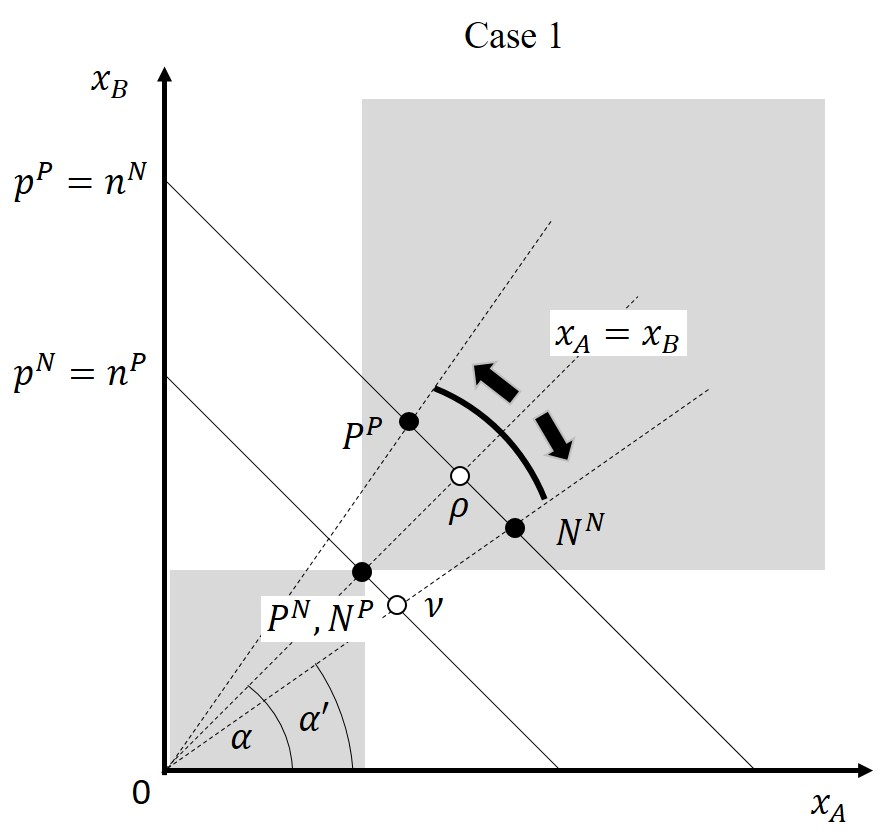
\includegraphics[scale=0.4]{figures/main_design_case_1.jpg}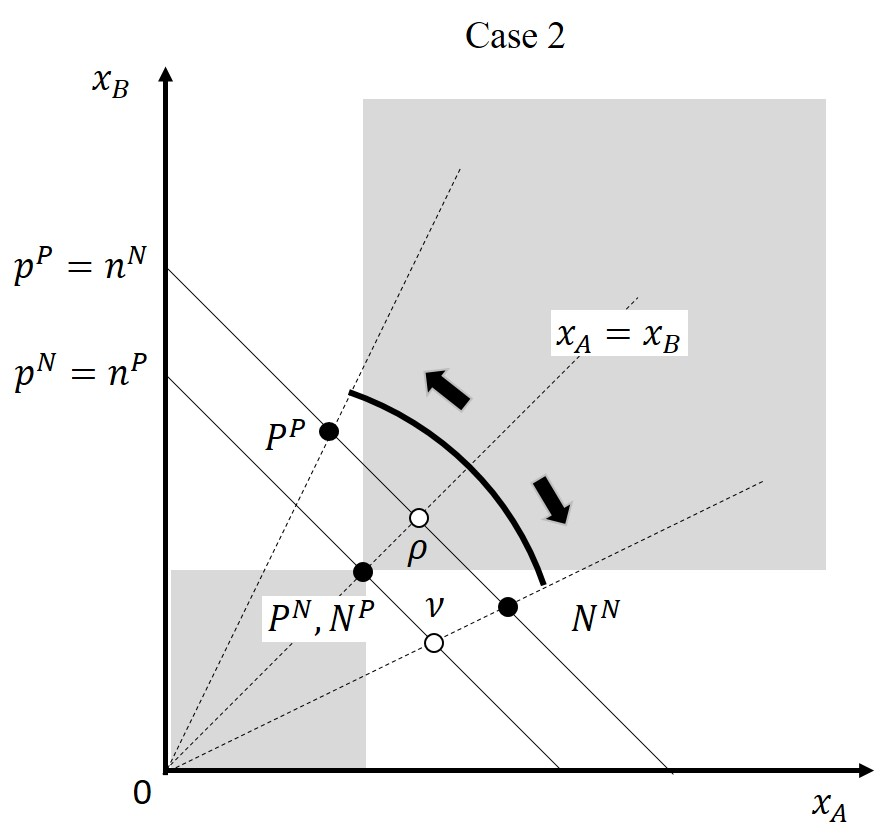
\includegraphics[scale=0.4]{figures/main_design_case_2.jpg}
   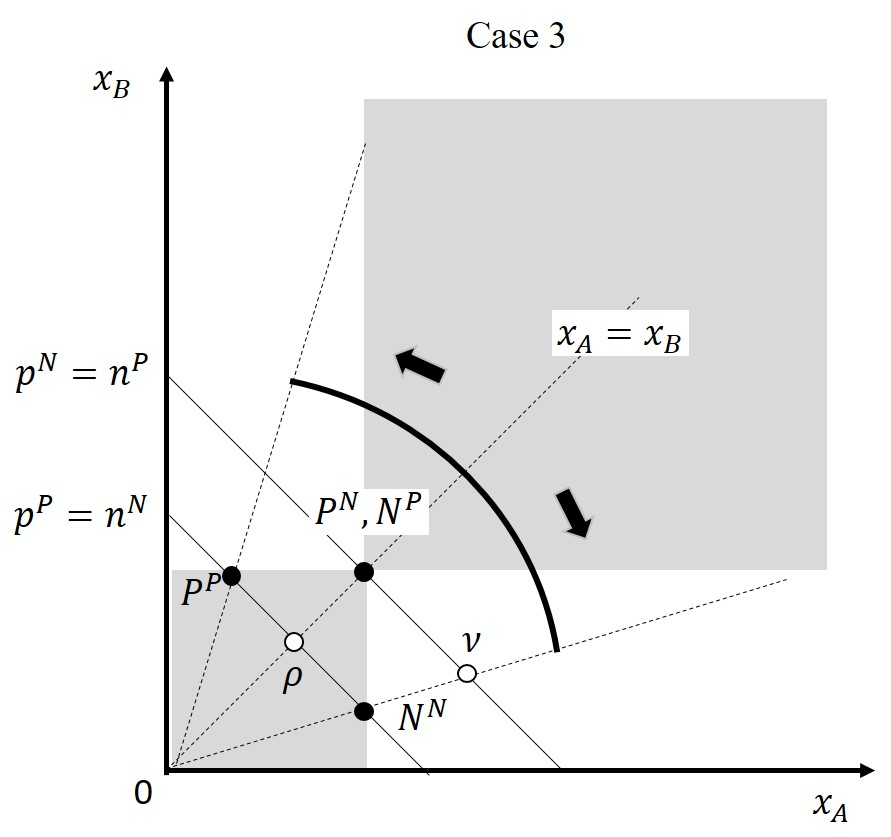
\includegraphics[scale=0.4]{figures/main_design_case_3.jpg}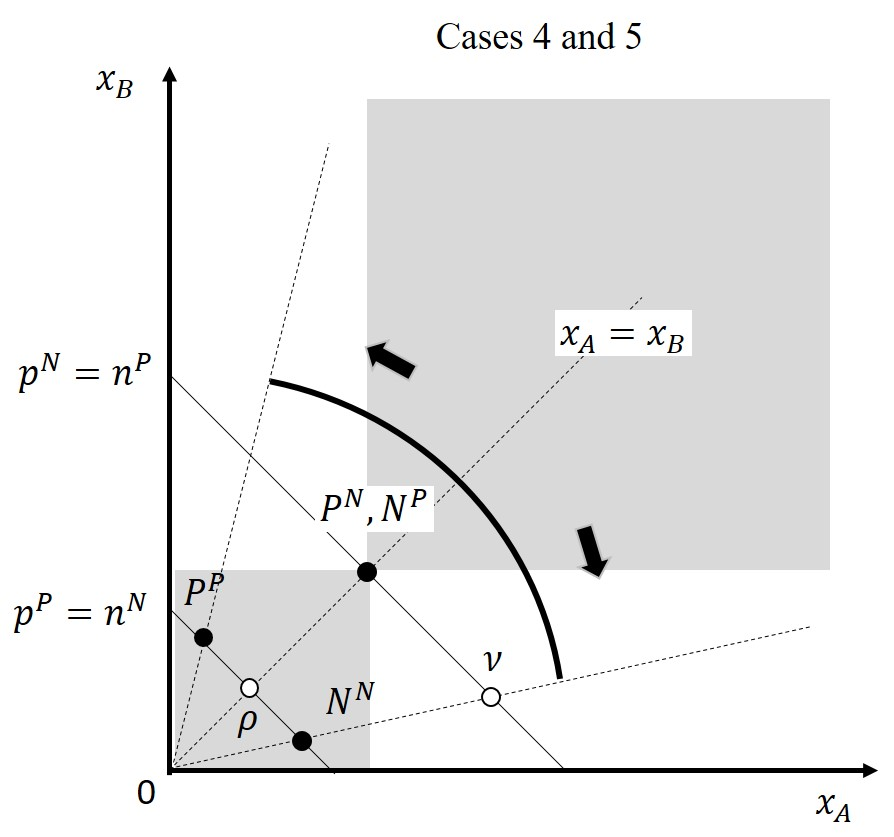
\includegraphics[scale=0.4]{figures/main_design_case_4.jpg}
   \begin{minipage}{12cm}
   \footnotesize
   \emph{The figure shows the parametrization of the vignette in a log-distribution diagram by case and scenario. $x_i^s$ is number of logs distributed to Person $i\in\{A,B\}$ in scenario $s\in\{N,P\}$. $P^s$ and $N^s$ are the distributions of need and productivity, and $n^s$ and $p^s$ are total need and total productivity that were presented to the participants. $P^N$ and $N^P$ are located on the $\alpha=45^\circ$ line of equality ($x_A=x_B$). $N^N$ is located on the $\alpha'$ degree line through the origin, and $P^P$ is located on the $90-\alpha'$ degree line through the origin. It is expected that participants pick the just distribution from the line $\overline{P^N\nu}$ in the Need Scenario and $\overline{P^P\rho}$ in the Productivity Scenario. Distributions in the grey shaded area at the top right of $P^N$ ($N^P$) involve a deficit (surplus) to both A and B. Distributions in the grey shaded area at the bottom left of $P^N$ ($N^P$) involve a surplus (deficit) to both A and B. Distributions in the white areas are mixed.}
   \caption{Study Design}
   \label{fig:design}
   \end{minipage}
\end{figure}
%
The parametrization of the vignettes enables studying the effect of the \textit{supply situation} (D$=$deficit, S$=$surplus, X$=$exact need satisfaction) and the source of heterogeneity on the distribution of logs among A and B. Figure \ref{fig:design} illustrates the design of the cases. Case 1, displayed in the top left diagram, introduces a situation where both A and B have a deficit of logs (DD) in the Need Scenario and a surplus of logs (SS) in the Productivity Scenario.\par
%
In the Need Scenario, total productivity is displayed as a straight ``supply'' line with intercept $p^N$. Point $P^N$ on this line marks the actual distribution of productivity. Total need is displayed as a straight ``demand'' line with intercept $n^N$. Point $N^N$ on this line marks the distribution of need. Since $N^N$ is located in the grey shaded area at the top right of $P^N$, both A and B have a deficit. And since $N^N$ is located to the right of the $45^\circ$ line of equality (where $x_A=x_B$), A is worse off than B because she has a bigger deficit.\par
%
Analogously, in the Productivity Scenario, total productivity is displayed as a straight line with intercept $p^P$, and point $P^P$ on this line marks the actual distribution of productivity. Total need is displayed as a straight line with intercept $n^P$, and point $N^P$ on this line marks the distribution of need. Since $P^P$ is located in the grey shaded area at the top right of $N^P$, both A and B have a surplus. And since $P^P$ is located to the left of the $45^\circ$ line of equality, A is worse off than B because she has a lower surplus. Hence, case 1 in the Productivity Scenario is a mirror image of case 1 in the Need Scenario where the source of heterogeneity and A's disadvantage is either need or productivity.\par
%
The other cases are constructed similarly. In case 2 in the top right diagram of Figure \ref{fig:design}, A has a deficit and B a surplus in the Need Scenario (point $N^N$ is in the area at the bottom right of $N^P$), and A has a surplus and B a deficit in the productivity scenario (point $P^P$ is in the area at the top left of $P^N$). Case 3 in the bottom left diagram shows a situation where A's need is either exactly satisfied or she has surplus, and where B has a surplus or her need is exactly satisfied, depending on the scenario. In cases 4 and 5, $N^N$ and $P^P$ are located in the grey shaded area at the bottom left of $P^N$ and $N^P$, respectively, and, hence, both A and B have a surplus in the Need Scenario or a surplus in the Productivity Scenario. Case 5 ``doubles'' case 4, has a slightly different parametrization, and was included to study participants' sensitivity towards need in more ``extreme'' situations. The results regarding this question will be reported in a different paper.\par
%
\subsection{Procedures}\label{sec:procedure}
%
Since participants received only a flat payment, we promoted internal validity by asking three control questions after the distribution task in order to make sure that the participants read the instructions carefully and actually understood the task. For the wording of the control questions, see Appendix \ref{sec:app_comprehension}. Only those who passed at least two out of three checks were included in the final analysis.\par
%
In order to control for participants' heterogeneity with regard to their socio-demo\-graphics and justice attitudes, we asked them, in a post-survey questionnaire, for their age, gender, and equivalent household net income and to state their support for three different distribution principles---need, equity, and equality (compare, for example, \citealt{skitka_allocating_1992} as well as \citealt{mitchell_judgments_1993}) as well as their evaluation of Person A's accountability for her situation on a 7-point Likert scale. We also assessed participants' perceived locus of control in a similar way (see \citealt{fong_social_2001} and \citealt{phares_internal-external_1975}) and collected information on participants' health status (dummy variables for being a smoker and suffering from a cardiovascular or metabolic disease). \cite{ubel_allocation_2001} found that smokers tend to punish unhealthy behavior regarding the need for transplant organs less often than participants who never smoked (also see \citealt{diederich_zur_2010}). Participants were also asked for their political orientations using a 7-point Likert scale ranging from 1 (most left-wing) to 7 (most right-wing), see Appendix \ref{sec:app_questions} for wordings.\par
%
The survey was programmed in oTree \citep{chen_otree_2016} and conducted online in September 2019. For reasons of external validity, participants were recruited via the private market research institute respondi. We used respondi's Online Access Panel which offers a quota sample of the German adult population. Our sample is a random sample of the Online Access Panel, stratified by the three characteristics gender, age, and equivalent household net income, with a sample-size of $N=200$ (for a breakdown of the sample by gender, age, and income, see Table \ref{tab:quota_demos} in Appendix \ref{sec:app_tables}). The sampling rates of these characteristics in our sample are representative of the adult German population. On the importance of a sample being representative if empirical research is considered as relevant for normative theory, see \cite{schwettmann_simple_2020}. Due to financial constraints, though, it was not possible to draw a larger sample that would potentially have captured more characteristics of the German population. The 200 participants who passed the control questions were paid a flat fee of 4.90 euro, equal to 9.80 euro per hour. Note that a further 203 persons started the survey but failed to pass the control questions. These persons were not asked any further questions and did not receive any payment. It was announced by respondi in the beginning of the study that failure to answer the control questions correctly would lead to exclusion from the study without being compensated. The control questions generated similar failure rates (Q1: 29\%, Q2: 31\%, Q3: 38\%). Participants who failed to pass the control questions did not differ from included participants by their stratification characteristics (gender: $\chi_1^2=0.517$, $p=0.526$; age: $\chi_4^2=5.083$, $p=0.279$; income: $\chi_4^2=3.447$, $p=0.486$). The enormous amount of dropouts shows that general population samples without performance-related incentives can potentially generate a lot of noise in the data. Hence, relatively strict exclusion criteria should be applied.\par
%
Before conducting the main study, we tested the efficacy of the vignette with respect to the accountability framing. All details of the pretest are reported in Appendix \ref{sec:app_pretest}. It clearly confirmed that participants attribute higher accountability to persons who disregard their doctor's warning.\par
%
\subsection{Working Hypotheses}\label{sec:hypotheses}
%
As explained above, participants were asked to distribute the logs between A and B according to what they thought to be most just. Let $x_i^s$ denote the number of logs distributed to person $i\in\{A,B\}$ in scenario $s\in\{N,P\}$. We assume that participants maximize the justice $J$ of the distribution $(x_A^s,x_B^s)$ subject to $x_B^s=p_A^s+p_B^s-x_A^s$ where the parametrization of the vignette by case and scenario with respect to need $(n_A^s,n_B^s)$, productivity $(p_A^s,p_B^s)$, and accountability treatment $T=\{low,high\}$ is given. Hence, the optimum number of logs distributed to person A is given by
%
\begin{equation}
x_A^{s\ast}=\arg\max J(x_A,p_A+p_B-x_A|n_A,n_B,p_A,p_B,T)\,.
\end{equation}
%
Since we study the justice views of laypersons in terms of participants' actual distribution choices $x_A^{s\ast}$, $J$ is not further specified or ``axiomatized''. For a comprehensive account of justice evaluation functions, see \citet{jasso_justice_1978} and \citet{jasso_distributive_2016}.\par
%
We consider two outcome measures of the experiment which both are based on $x_A^{s\ast}$. Since the total number of logs available differs from case to case and between the scenarios, we normalize $x_A^{s\ast}$ by Person A's and Person B's total productivity, $p^s$, to obtain the first outcome measure, namely, the \textit{share of logs distributed to Person A}:
%
\begin{equation}
\mbox{logshare}_A^s=\frac{x_A^{s\ast}}{p^s}\,.
\end{equation}
%
For example, point $P^N$ in case 1 in Figure \ref{fig:design} shows a situation where the logs are distributed exactly according to productivity. Thus, we have $\mbox{logshare}_A^N=0.5$ and $\tan^{-1}(x^N_B/x^N_A)=\tan^{-1}(1000/1000)=45^\circ=\alpha$. Analogously, point $\nu$ where the line through the origin $\overline{0N^N}$ and the ``supply'' line $p^N$ intersect, shows a situation where the logs are distributed proportional to need. Thus, we have $\mbox{logshare}_A^N=0.6$ and $\tan^{-1}(800/1200)=\alpha'=34^\circ$.\par
%
The second outcome measure is the \textit{normalized deviation from the equal split} in favor of Person A:
%
\begin{equation}
\mbox{deviation}_A^s=\left\{\begin{array}{ll} \frac{\mbox{logshare}_A^s-0.5}{n_A^s/n^s-0.5} & \mbox{(Need Scenario)} \\
\frac{0.5-\mbox{logshare}_A^s}{0.5-p_A^s/p^s} & \mbox{(Productvitiy Scenario)}\,.
\end{array}
\right.
\end{equation}
%
The allocation that distributes resources equally---the equal split---has been demonstrated to serve as a natural \textit{reference point} or \textit{social norm} for
bargaining processes (compare, for example, \citealt{yaari_dividing_1984}, \citealt{dawid_robust_2006}, as well as \citealt{andreoni_social_2009}). In bargaining experiments, participants frequently choose equal-split allocations even though they are Pareto dominated \citep{herreiner_inequality_2010}. However, in social choice experiments, only a minority of participants still opts for the equal split when objective reasons like need differences speak in favor of an unequal distribution \citep{gaertner_empirical_2012}. Hence, participants' sense of justice is reflected in the deviation from the equal split.\par
%
We have $\mbox{deviation}_A^s=0$ (equal split) when participants think that heterogeneity among A and B is irrelevant. In Figure \ref{fig:design}, equal-split distributions are located on the $45^\circ$ line which goes through points $N^P$ (equal productivity) and $P^N$ (equal need). We have $\mbox{deviation}_A^s>0$ when participants think that A should be compensated for her disadvantage due to greater need (clockwise rotation) or smaller productivity (counterclockwise rotation). Observations that do not meet the condition $0\le\mbox{deviation}_A^s\le1$, that is, choices that make A's situation even worse than it is or make A better off than B are considered as noise in the analysis.\par
%
We expect that, on average, participants distribute more than A's productivity share and less than A's need share to her, because they think it is just to \textit{partially} compensate A for her disadvantage. Consequently, $\mbox{logshare}_A^s$ in the Productivity Scenario is smaller than in the Need Scenario because A's need share in the Productivity Scenario is 50\% (the upper bound for $\mbox{logshare}_A^P$), and her productivity share in the Need Scenario is also 50\% (the lower bound for $\mbox{logshare}_A^N$). Hence, the deviation from the equal split is between zero and one. Put into graphs, we expect participants to pick the just distributions from the line $\overline{P^N\nu}$ in the Need Scenario and the line $\overline{P^P\rho}$ in the Productivity Scenario in Figure \ref{fig:design}.
%
\begin{Hypothesis}[Partial Compensation]
Participants compensate Person A partially for her disadvantage: $p_A^s/p^s<\mbox{logshare}_A^s<n_A^s/n^s$. Partial compensation implies that
$\mbox{logshare}_A^P<0.5<\mbox{logshare}_A^N$ and $0<\mbox{deviation}_A^s<1$.
\end{Hypothesis}
%
\par
%
We expect that participants' willingness to compensate Person A for her disadvantage is diminished by high accountability. Hence, participants distribute fewer logs to A and they favor smaller (greater) deviations from the equal split in the Need Scenario (Productivity Scenario).
%
\begin{Hypothesis}[Accountability] The just distribution of logs depends on A's accountability such that
\begin{enumerate}
\renewcommand{\labelenumi}{\alph{enumi})}
\item $\mbox{logshare}_A^s(low)>\mbox{logshare}_A^s(high)$,
\item $\mbox{deviation}_A^N(low)>\mbox{deviation}_A^N(high)$ and $\mbox{deviation}_A^P(low)<\mbox{deviation}_A^P(high)$.
\end{enumerate}
\end{Hypothesis}
%
\par
%
If $J$ is homogeneous in the number of logs, A's just share of logs is determined by her need share and her productivity share, and not by total need and total productivity. Let $\alpha^s=\tan^{-1}(x_B^{s\ast}/x_A^{s\ast})$ denote the angle of the line through the origin that contains all just distributions. Since Need Scenario and Productivity Scenario are mirror images of each other, we expect $45^\circ-\alpha^N=\alpha^P-45^\circ$ which is equivalent to $\mbox{logshare}_A^N=1-\mbox{logshare}_A^P$. This implies that the just deviation from the equal split is independent of the scenario as indicated by the black arrows in Figure \ref{fig:design}.
%
\begin{Hypothesis}[Scenario] Disadvantages that are due to greater need and smaller productivity are treated symmetrically, that is,
$\mbox{logshare}_A^N=1-\mbox{logshare}_A^P$ and\linebreak $\mbox{deviation}_A^N=\mbox{deviation}_A^P$.
\end{Hypothesis}
%
\par
%
However, one could argue that the cognitive perception of the scenarios differs because the equal split is seen as a reference point (\citealt{trueblood_reference_2015}). Loss averse participants might find compensating A less justified when her disadvantage is due to lower contribution (negative domain, reduction of a loss for A) than when her disadvantage is due to greater need (positive domain, gain for A). Hence, there could be a gain-loss domain effect (\citealt{tversky_loss_1991}, also see \citealt{weis_needs_2017}) that would imply $\mbox{deviation}_A^P>\mbox{deviation}_A^N$. Moreover, there could also be an \textit{interaction effect} between scenario framing and accountability treatment.\par
%
As can be seen in Table \ref{tab:cases} and Figure \ref{fig:design}, the five cases differ by their supply situation. Figure \ref{fig:design} shows that $P^N$ and $N^P$ remain constant, while $N^N$ and $P^P$ are obtained from systematically changing both relative \textit{inequality} in productivity or need (visualized by the angles of the dashed lines through $N^N$ and $P^P$ to the line of equality) and total need or total productivity (visualized by the ``demand'' and ``supply'' lines). Hence, the study design does not allow the separation of both possible effects on the just distribution of logs. Keeping relative inequality constant would have led to very small absolute need and productivity differences in cases where $N^N$ and $P^P$ are located in the grey shaded area at the bottom left of $P^N$ and $N^P$. Hence, we decided to additionally increase relative inequality among A and B.\par
%
In order to deal with this problem, we first assume that the absolute supply situation in terms of A having a deficit or surplus (the location of the ``demand'' and ``supply'' lines) does not affect participants' justice considerations. Hence, in the Need Scenario, we expect that the share of logs that is distributed to A \textit{increases} in relative inequality when moving from case 1 to 5 because point $\nu$ moves outward on the line of just distributions $\overline{P^N\nu}$ and $\alpha'$ decreases. The opposite applies to the Productivity Scenario where $P^P$ moves outward on the line of just distributions $\overline{P^P\rho}$ and $90-\alpha'$ increases. Hence, in the Need Scenario (Productivity Scenario), we hypothesize that participants distribute relatively more (less) logs to A when a case exhibits greater inequality among A and B. Since the deviation from the equal split is normalized by the difference between A's need share and her productivity share (the length of $\overline{P^N\nu}$ and $\overline{P^P\rho}$), we expect it to be independent of the supply situation.
%
\begin{Hypothesis}[Supply Situation] Let $y,z\in\{1,2,3,4,5\}$ denote the number of the case where $y<z$ and cases with lower numbers exhibit less inequality (with respect to need or productivity) among A and B, then we have $\mbox{logshare}_A^N(z)-\mbox{logshare}_A^P(z)>\mbox{logshare}_A^N(y)-\mbox{logshare}_A^P(y)$ and $\mbox{deviation}_A^s(y)=\mbox{deviation}_A^s(z)$.
\end{Hypothesis}
%
\par
%
If the absolute supply situation matters for the distribution of logs, it is likely to have a dampening effect in the Need Scenario (A receives relatively less, $\alpha'$ decreases less) because increasing inequality is combined with an improving absolute supply situation (Person A starts with a deficit and ends up with a surplus). It is also likely to have a dampening effect in the Productivity Scenario (A receives relatively more, $90-\alpha'$ increases less) because increasing inequality is combined with a worsening absolute supply situation (Person A starts with a surplus and ends up with a deficit). Hence, the two scenario differences in \textbf{H4} might get smaller, but the effect of increasing inequality should remain.\par
%
\section{Results}\label{sec:results}
%
We begin the presentation of the results with participants' responses to the accountability question posed in the post-survey questionnaire. In order to interpret the results of this study in terms of Person A's accountability for her disadvantage, it is necessary to establish that the accountability framing actually worked. As noted in the previous section, the vignette design had already been successfully tested in a pretest, though with a student sample. Next, in Subsection \ref{sec:distribution}, we test our working hypotheses by studying participants' \textit{average} distribution choices. In Subsection \ref{sec:choices}, we then turn to participants' \textit{individual} distribution choices, and we identify different distribution principles that participants consistently applied in order to distribute the logs of wood to Persons A and B.\par
%
\subsection{Accountability Judgments}\label{sec:accountability}
%
Figure \ref{fig:responsibility} shows participants' mean judgment of Person A's accountability for her greater need and her lower productivity on a 7-point Likert scale. A two-tailed t-test confirms that, in both scenarios, the bar representing the High Accountability Treatment is significantly larger than the one representing the Low Accountability Treatment (Need Scenario, High Accountability Treatment: mean~$=5.00$ (90\% CI~$=[ 4.72,5.28]$), Low Accountability Treatment: mean~$=4.04$ (90\% CI~$=[3.75,4.34]$), mean difference~$=0.96$ (90\% CI~$=[0.55, 1.36]$), $p\le0.01$; Productivity Scenario, High Accountability Treatment: mean~$=5.16 $ (90\% CI~$=[4.88,5.43]$), Low Accountability Treatment: mean~$=3.98$ (90\% CI~$=[3.68,4.28]$), mean difference~$=1.18$ (90\% CI~$=[0.78,1.58]$), $p\le0.01$; two-sample two-tailed t-test, between-participants treatment). Hence, as already suggested by the pretest, the vignette was effective for inducing a low and a high accountability frame in participants with respect to Person A's disadvantage.\par
%
Moreover, Figure \ref{fig:responsibility} indicates that there is no significant difference in participants' mean judgment of Person A's accountability between Need and Productivity Scenario. A pairwise two-tailed t-test cannot reject the null hypothesis of equality of the mean accountability judgment (High Accountability Treatment, Need Scenario vs. Productivity Scenario: mean difference~$= -0.16$ (90\% CI~$=[-0.31, 0.02]$), $p = 0.104$; Low Accountability Treatment, Need Scenario vs. Productivity Scenario: mean difference~$=0.07$ (90\% CI~$=[-0.18, 0.31]$), $p = 0.659$; paired-sample two-tailed t-test, within-participants treatment). Hence, we conclude that it did not matter to the participants whether A's disadvantage was caused by need or productivity differences.\par
%
\begin{figure}[ht!]
   \centering
   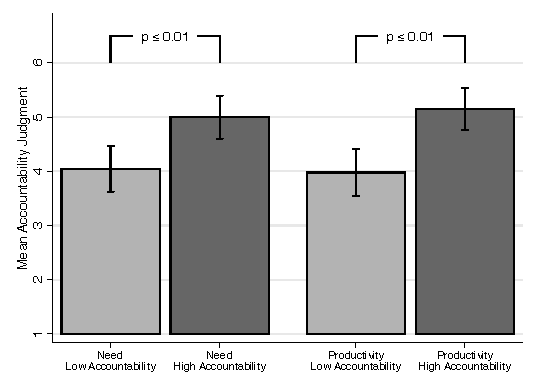
\includegraphics[scale=0.7]{figures/main_accountability.pdf}
   \begin{minipage}{10cm}
   \footnotesize
   \emph{The figure shows participants' mean judgment of Person A's accountability for her greater need (lower productivity) in the Low (High) Accountability Treatment using a 7-point Likert scale. Larger numbers mean greater accountability. The grey (white) bars represent $N=91$ ($N=109$) observations each. Error bars represent 90\% confidence intervals for the mean. $p$ value of a two-tailed two-sample t-test (between-participants).}
   \caption{Mean Accountability Judgment by Treatment and Scenario}
   \label{fig:responsibility}
   \end{minipage}
\end{figure}
%
\subsection{Average Distribution Choices}\label{sec:distribution}
%
In this subsection, we turn to our main interest, namely, the impact of scenario and accountability treatment on the just distribution of logs. We also analyze how the supply situation affects the distribution of logs. The following analyses of $\mbox{logshare}_A^s$ and $\mbox{deviation}_A^s$ are based on 2000 distribution choices (10 per participant). Note that only 208 distribution choices (10.4\%) do not meet the condition $0\le\mbox{deviation}_A\le1$.\par
%
\subsubsection*{Means}
%
Figure \ref{fig:distribution} displays $\mbox{logshare}_A^s$ as a bar chart (left panels) and $\mbox{deviation}_A^s$ as a range plot (right panels). The top panels show the distribution of logs by treatment and scenario; the middle (bottom) panels show the distribution of logs in the Need Scenario (Productivity Scenario) by treatment and case. Means, standard errors, cases numbers, and t-tests can be seen in Tables \ref{tab:share_means} and \ref{tab:dev_means} in Appendix \ref{sec:app_tables}.\par
%
\begin{figure}[ht!]
   \centering
   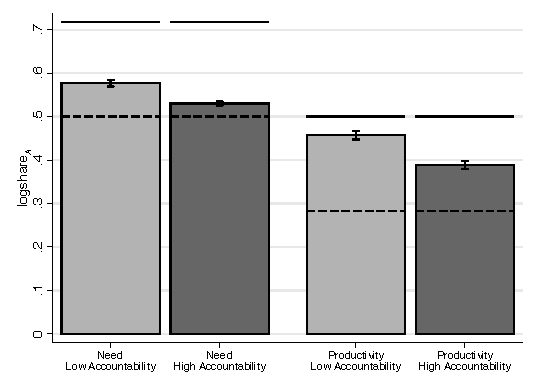
\includegraphics[scale=0.4]{figures/main_mean_share.pdf}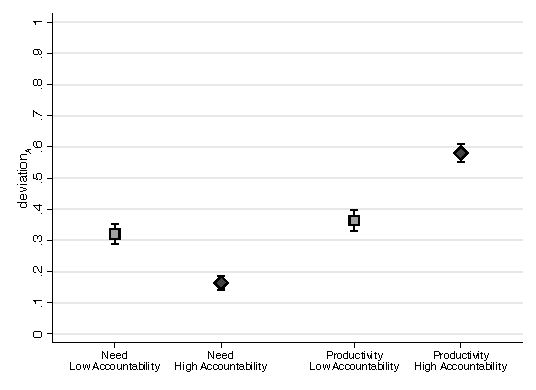
\includegraphics[scale=0.4]{figures/main_mean_deviation.pdf}
   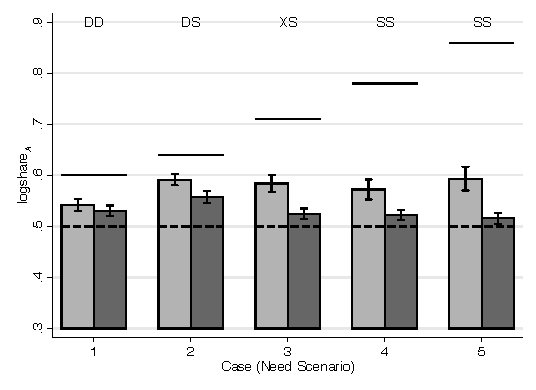
\includegraphics[scale=0.4]{figures/main_share_need.pdf}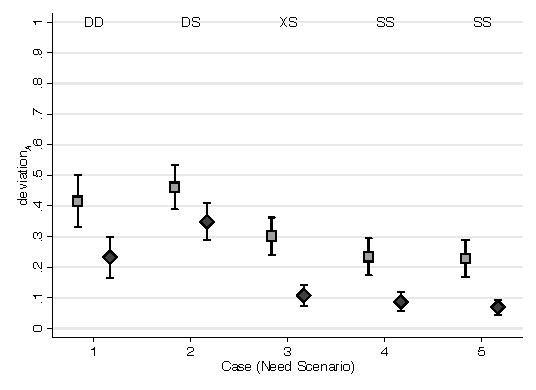
\includegraphics[scale=0.4]{figures/main_deviation_need.pdf}
   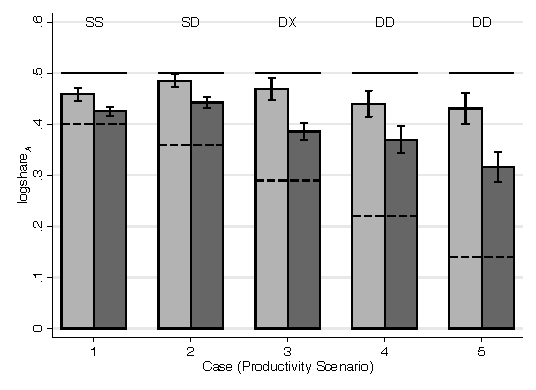
\includegraphics[scale=0.4]{figures/main_share_productivity.pdf}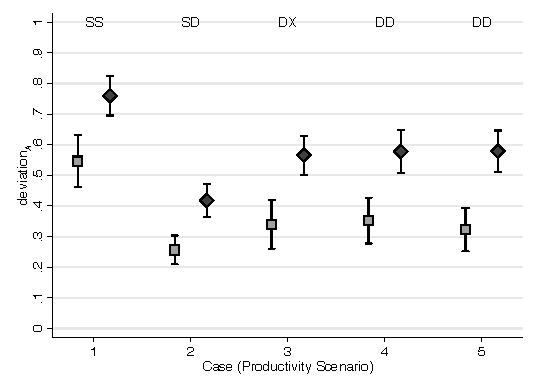
\includegraphics[scale=0.4]{figures/main_deviation_productivity.pdf}
   \begin{minipage}{12cm}
   \footnotesize
   \emph{The bars show the mean share of logs distributed to Person A ($\mbox{logshare}_A^s$) by scenario and treatment (top left panel), by treatment and case in the Need Scenario (middle left panel), and by treatment and case in the Productivity Scenario (bottom left panel). The solid (dashed) line indicates Person A's need (productivity) share. The range plots show the mean relative deviation from the equal split ($\mbox{deviation}_A^s$) by scenario and treatment (top right panel), by treatment and case in the Need Scenario (middle left panel), and by treatment and case in the Productivity Scenario (bottom left panel). Error bars represent 90\% confidence intervals for the mean. For case numbers, means, standard errors, and t-tests see Tables \ref{tab:share_means} and \ref{tab:dev_means} in Appendix \ref{sec:app_tables}. Supply situation of A and B: D$=$deficit, S$=$surplus, X$=$exact need satisfaction.}
   \caption{Distribution of Logs}
   \label{fig:distribution}
\end{minipage}
\end{figure}
%
Concerning the partial compensation hypothesis (\textbf{H1}), the bar charts show as hypothesized that participants \textit{on average} distributed significantly more logs to Person A than her productivity share and significantly less than her need share in all scenarios, treatments, and cases. Consequently, $\mbox{logshare}_A$ exceeds 50\% in the Need Scenario and falls below 50\% in the Productivity Scenario. The range plots of $\mbox{deviation}_A$ lie between 0 and 1.\par
%
The accountability hypothesis (\textbf{H2}) is clearly confirmed by the data, too. As regards the share of logs distributed to A, the treatment effect of high accountability is significant in all cases except for case 1 in the Need Scenario (see Table \ref{tab:share_means}). As regards the deviation from the equal split, the treatment effect is also significant (except for case 1), and it is negative in the Need Scenario and positive in the Productivity Scenario (see Table \ref{tab:dev_means} in the Appendix) as hypothesized.\par
%
The hypotheses concerning the symmetry of the scenarios (\textbf{H3}) and the impact of the supply situation (\textbf{H4}) are tested using regression analysis. Test results are reported in the following paragraphs.\par
%
\begin{figure}[ht!]
   \centering
   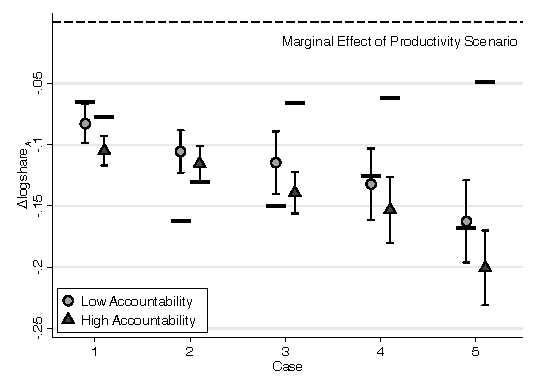
\includegraphics[scale=0.4]{figures/main_marg_share_scenario.pdf}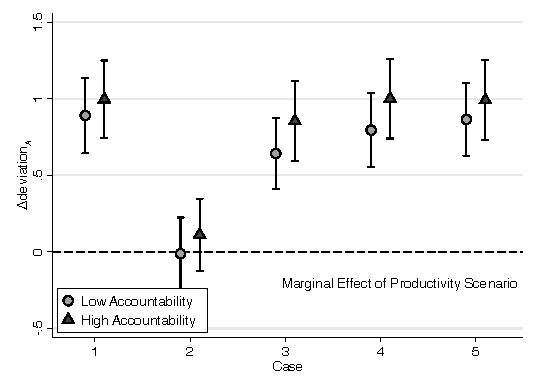
\includegraphics[scale=0.4]{figures/main_marg_deviation_scenario.pdf}
   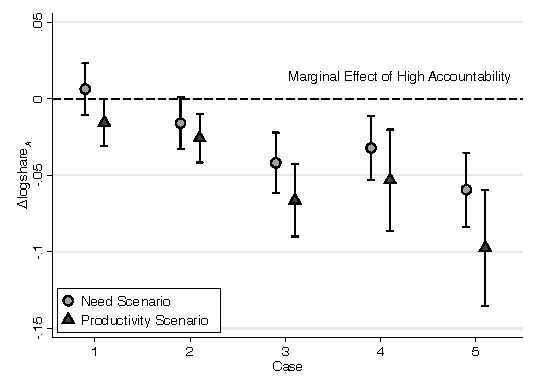
\includegraphics[scale=0.4]{figures/main_marg_share_case.pdf}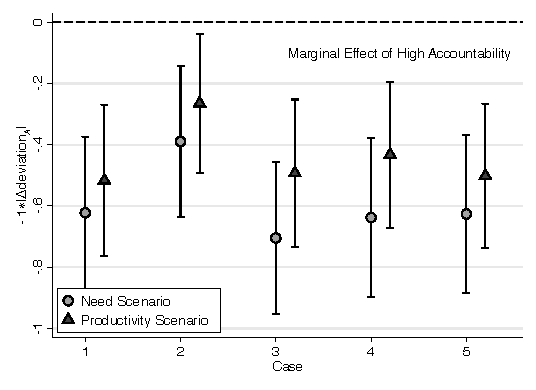
\includegraphics[scale=0.4]{figures/main_marg_deviation_case.pdf}
   \begin{minipage}{\linewidth}
   \footnotesize
   \emph{Left panels: marginal effect ($\Delta\mbox{logshare}_A^s$) of the Productivity Scenario (top) and of high accountability (bottom) estimated from a GLS random effects panel regression. The thick lines in the top left panel indicate the reference values for testing symmetry of the scenarios. Right panels: marginal effect ($\Delta\mbox{deviation}_A^s$) and negative absolute marginal effect ($-1\times|\Delta\mbox{deviation}_A^s|$) of the Productivity Scenario (top) and the High Accountability Treatment (bottom) estimated from a tobit random effects panel regression. Error bars represent 90\% confidence intervals for the mean.}
   \caption{Marginal Effects}
   \label{fig:marginaleffect}
\end{minipage}
\end{figure}
%
\subsubsection*{Marginal Effects of Scenario and Supply Situation}
%
The analysis of means controls neither for participants' socio-demographics and attitudes nor for potential ordering effects. Hence, we perform regression analysis. All statistical details and tables are given in Appendix \ref{sec:regression}. The estimated marginal effects of scenario, supply situation, and accountability treatment are displayed in Figure \ref{fig:marginaleffect}.\par
%
First, we turn to the marginal effects of scenario and supply situation on the \textit{share of logs}. The top left panel of Figure \ref{fig:marginaleffect} displays the marginal effect of the Productivity Scenario (the Need Scenario is the benchmark case) on the share of logs distributed to A by accountability treatment and case. All marginal effects are negatively significant as hypothesized by the partial compensation hypothesis (\textbf{H1}). There is no difference between the accountability treatments with respect to the marginal effect of the Productivity Scenario, except for case 1 (see Table \ref{tab:marginalscen} in Appendix \ref{sec:regression}).\par
%
A pairwise comparison of the marginal effect of the Productivity Scenario by case shows that the negative impact of the Productivity Scenario in cases 4 and 5 is significantly greater than in case 1. This confirms the supply-situation hypothesis (\textbf{H4}) which holds that increasing inequality with respect to need or productivity among A and B causes greater differences of A's just share of logs between the scenarios (see the top panel of Table \ref{tab:marginalcase} in Appendix \ref{sec:regression}, significance levels are corrected for multiple hypotheses testing using the Bonferroni correction).\par
%
In order to test the symmetry of the scenarios (\textbf{H3}), we first compute $\mbox{logshare}_A^N$ and $\mbox{logshare}_A^P$, and then we test $\mbox{logshare}_A^N=1-\mbox{logshare}_A^P$. In the top left panel of Figure \ref{fig:marginaleffect}, the thick lines indicate the reference values for testing symmetry of the scenarios. As can be seen in Figure \ref{fig:marginaleffect}, in the Low Accountability Treatment, symmetry cannot be rejected, except for cases 2 and 3 where the positive difference of A's share of logs from 50\% in the Need Scenario exceeded the negative difference of her share of logs from 50\% in the Productivity Scenario. In the High Accountability Treatment, symmetry is clearly rejected (except for case 2). Just distributions are ``biased'' in the direction discussed in Subsection \ref{sec:hypotheses}; participants deviated more from the equal-split distribution when A's disadvantage was due to lower productivity than when it was due to greater need (see Table \ref{tab:symmetry} in Appendix \ref{sec:regression}).\par
%
The top right panel of Figure \ref{fig:marginaleffect} displays the marginal effect of the Productivity Scenario on the \textit{deviation from the equal split} by accountability treatment and case (also see Table \ref{tab:marginalscen} in Appendix \ref{sec:regression}). Except for case 2 in both treatments as well as cases 1 and 3 in the High Accountability Treatment, all marginal effects are positively significant, thereby rejecting the hypothesis that disadvantages due to greater need and smaller productivity are treated symmetrically (\textbf{H3}). High accountability dampens the asymmetry because the share of respondents who are not all willing to compensate Person A for her disadvantage is relatively high in both scenarios.\par
%
Case 2 differs significantly from all other cases. In this regard, we have to qualify our previous conclusion that \textbf{H4} ($\mbox{deviation}_A^s(y)=\mbox{deviation}_A^s(z)$) is supported by the data. Remember that case 2 involves a deficit for A and a surplus for B in both scenarios. In Subsection \ref{sec:choices}, we show that some participants applied a specific distribution principle in this mixed supply situation, which we call ``net split''.\par
%
\subsubsection*{Marginal Effect of Accountability}
%
Now, we turn to the marginal effect of \textit{accountability} (for statistical details, see Tables \ref{tab:marginalaccount} and \ref{tab:marginalcase} in Appendix \ref{sec:regression}). The bottom left panel of Figure \ref{fig:marginaleffect} displays the marginal effect of the High Accountability Treatment on the share of logs distributed to A (the Low Accountability Treatment is the benchmark case). Except for cases 1 and 2 in the Need Scenario, all marginal effects are negatively significant. The figure also shows that high accountability had a significantly greater negative impact in cases 4 and 5 than in case 1. Hence, the supply situation in terms of greater inequality among A and B caused a greater accountability effect with respect to the just share of logs distributed to A.\par
%
According to \textbf{H2}, we also expect $\Delta\mbox{deviation}_A<0$ in the Need Scenario and\linebreak $\Delta\mbox{deviation}_A>0$ in the Productivity Scenario. Hence, we display $-1\times |\Delta\mbox{deviation}_A|$ in the bottom right panel of Figure \ref{fig:marginaleffect} to ease visual comparisons. The bottom right panel displays the marginal effect of the High Accountability Treatment by scenario and case. As expected, the marginal effects are negatively significant (except for case 1 of the Need Scenario). There is no difference between the scenarios and there are case differences similar to the share of logs. In summary, the negative effect of high accountability is clearly confirmed (\textbf{H2}).\par
%
\subsubsection*{Control Variables}
%
Next, we address the \textit{control variables} (for statistical details, see Table \ref{tab:regression_share_cov} in Appendix \ref{sec:regression}). Participants with higher equivalent household net incomes were willing to allocate a greater share of logs to Person A. Among the health-related variables, only the smoker dummy exhibits a significant positive coefficient in the regressions on $\mbox{logshare}_A$ (and a negative coefficient in the regessions on $\mbox{deviation}_A$), which may point to a ``solidarity effect'' among smokers.\par
%
The covariates that capture participants' support for different distribution principles are significant in all regressions on the share of logs distributed to A. Participants who think that need is an important criterion of distributive justice distributed more logs to A and chose greater deviations from the equal split. Participants who think that equity is an important criterion of justice distributed less to A and, also, chose greater deviations from the equal split. Participants who show stronger support for equality gave more to A and, naturally, tolerated only smaller deviations from the equal split. The positive coefficient of the political-attitude variable indicates that people who place themselves rather on the right side of the political spectrum made less equal distribution choices.\par
%
Each participant submitted two accountability judgments---one for the Need Scenario and one for the Productivity Scenario. As can be seen in the bottom row of Table \ref{tab:regression_share_cov} in Appendix \ref{sec:app_tables}, the accountability judgments do not have a significant impact on average distribution choices ($\mbox{logshare}_A^s$ and $\mbox{deviation}_A^s$) when the accountability judgment enters the regression model as a differential intercept. Beyond that, it would be interesting to analyze whether the size of the accountability effect ($\Delta\mbox{logshare}_A^s$ and $-1\times|\Delta\mbox{deviation}_A^s|$) depends on within-subjects \textit{differences} between the accountability judgments of the two treatments in a given scenario. However, since participants were assigned to either the Low Accountability Treatment or the High Accountability Treatment, this analysis cannot be performed with our between-subjects design.\par
%
\subsection{Individual Distribution Choices}\label{sec:choices}
%
In this subsection, we look at participants' individual distribution choices. First, we group the five choices made by each participant in each scenario into several mutually exclusive categories according to the share of logs distributed to Person A. In the Need Scenario, the choice categories correspond to the following distribution principles: ``less'' than the equal split ($\mbox{logshare}_A^N<0.5$), ``equal split'' ($\mbox{logshare}_A^N=0.5$), ``partial compensation'' ($0.5<\mbox{logshare}_A^N<n_A^N/n^N$), A receives her ``need share'' ($\mbox{logshare}_A^N=n_A^N/n^N$), and A receives ``more'' than her need share ($\mbox{logshare}_A^N>n_A^N/n^N$). In the Productivity Scenario, the categories correspond to the following distribution principles: A receives ``less'' than her productivity share ($\mbox{logshare}_A^P<p_A^P/p^P$), A receives her ``productivity share'' ($\mbox{logshare}_A^P=p_A^P/p^P$), ``partial compensation'' ($p_A^P/p^P<\mbox{logshare}_A^P<0.5$), ``equal split'' ($\mbox{logshare}_A^P=0.5$), and ``more'' than the equal split ($\mbox{logshare}_A^P>0.5$). With regard to the exact distribution principles ``need share'', ``productivity share'', and ``equal split'', we tolerate that $\mbox{logshare}_A^s$ deviates 1 percentage point from the respective target value in order to account for typos and small rounding errors. Second, we identify participants who consistently applied the same distribution principle across all cases within a scenario.\par
%
\begin{figure}[ht!]
   \centering
   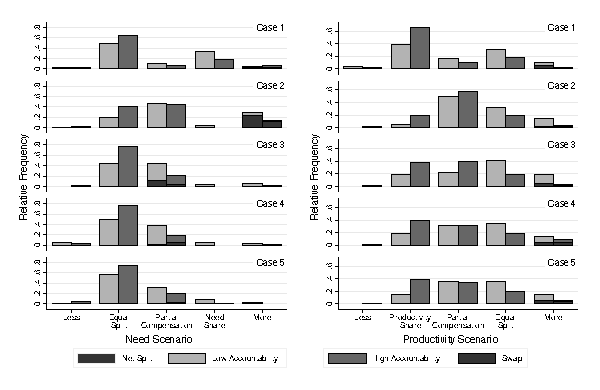
\includegraphics[scale=1]{figures/main_types_1.pdf}
   \begin{minipage}{10cm}
   \footnotesize
   \emph{The bars show the relative frequency of five distribution principles by case and scenario. Dark-shaded bars represent the share of ``Net split[s]'' (A and B receive the logs of wood they need plus/minus half of the oversupply/undersupply) and ``Swap[s]'' (A receives $(1-p_A^P/p^P)$, B receives $p_A^P/p^P$) in the respective category.}
   \caption{Relative Frequency of Distribution Principles by Case and Scenario}
   \label{fig:histogram}
\end{minipage}
\end{figure}
%
Figure \ref{fig:histogram} shows the relative frequency of individual choices that conform with one of the distribution principles by case and scenario. Grey (white) bars refer to the Low (High) Accountability Treatment. In the Need Scenario, equal split, partial compensation, and need share make up 89\% of all choices in the Low Accountability Treatment and 92\% in the High Accountability Treatment. Interestingly, participants almost never distributed logs of wood in exact accordance with A's need share (except for case 1 which depicts a situation of severe undersupply). A comparison of participants' distribution choices between the accountability treatments shows a clear shift towards the equal split when Person A is highly accountable for her disadvantage. The overall share of equal-split choices increases from 44\% to 66\% ($\chi^2_1=49.993$, $p\le0.01$). Increasing inequality from case 1 to case 5 does not intensify the effect of high accountability on the share of equal splits, however.\par
%
The dark shaded bars indicate the share of choices in the respective category that are also compatible with a distribution principle that might be called ``net split''. Here, A and B receive the absolute number of logs they need plus (or minus) half of the oversupply (or undersupply). Although the net split is an unusual distribution principle, 8\% of all choices in the Low Accountability Treatment and 5\% in the High Accountability Treatment are in line with the net-split principle, and it is particularly prevalent in the ``mixed supply'' case 2 (23\% vs.~12\%). Though we can conceive distribution principles which are perhaps more sophisticated than the ones displayed in the figure, other principles did not play a significant role in terms of having been chosen more than once or twice in the Need Scenario.\par
%
The right panel of Figure \ref{fig:histogram} shows a slightly different picture for the Productivity Scenario. 85\% of the choices in the Low Accountability Treatment and 94\% of the choices in the High Accountability Treatment distribute A's productivity share to her, compensate her partially, or split the logs equally among A and B. The distribution of the choices to the categories is more balanced, however. There is a clear shift from equal split and partial compensation towards A's productivity share in the High Accountability Treatment. The overall share of equal-split choices decreases from 35\% to 19\% ($\chi^2_1=33.035$, $p\le0.01$). As in the Need Scenario, there is no significant interaction between the size of the need gap and the marginal effect of high accountability on the share of equal splits. Moreover, there is a striking number of choices (14\% vs.~5\%) which distribute more than 50\% of the logs to A (though she has the same need as B and lower productivity than her). Many of these choices can be explained by the ``swap'' principle (displayed by the dark-shaded bars in the figure): A receives $(1-p_A^P/p^P)=p_B^P/p^P$\% of the logs and B $p_A^P/p^P=(1-p_B^P/p^P)$\%. Note that, in the Productivity Scenario, the net-split principle coincides with the equal split because A and B have equal need of logs.\par
%
\begin{figure}[ht!]
   \centering
   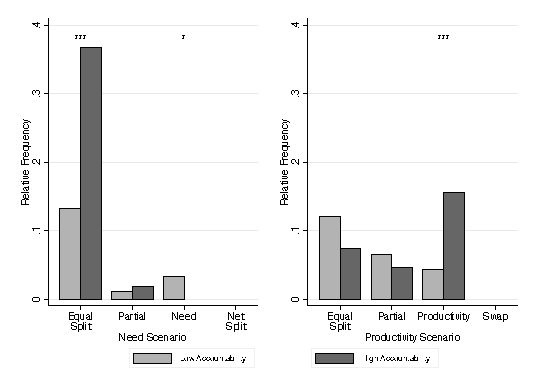
\includegraphics[scale=0.7]{figures/main_types_2.pdf}
   \begin{minipage}{10cm}
   \footnotesize
   \emph{The bars show the relative frequency of participants who consistently applied the same distribution principle across all cases by distribution principle and scenario. Asterisks denote significance levels of a $\chi^2$ test: $^{*}p\le0.10$, $^{**}p\le0.05$, $^{***}p\le0.01$.}
   \caption{Relative Frequency of Consistent Participants by Distribution Principle and Scenario}
   \label{fig:histogram_types}
\end{minipage}
\end{figure}
%
Finally, we turn to participants who consistently applied the same distribution principle across all five cases within a scenario. In Figure \ref{fig:histogram_types}, we focus on the four most important distribution principles according to their choice frequencies in the scenarios (Need Scenario: equal split, partial compensation, A's need share, and net split; Productivity Scenario: equal split, partial compensation, A's productivity share, and swap). The number of participants sticking to one of these distribution principle \textit{across all cases} is 17.6\% (low accountability) and 38.5\% (high accountability) in the Need Scenario; 24.2\% (low accountability) and 29.4\% (high accountability) in the Productivity Scenario. Considering six monistic distribution principles, \cite{meyer_individual_2019} found that across several experiments 37\% of the subjects always chose in line with the \textit{same} distribution principle. In five experiments that also involved need as a distribution principle, up to 18\% chose the need principle.\par
%
In the Need Scenario, 37\% of the participants consistently distributed logs to A and B according to the equal-split principle, when A was highly accountable for her disadvantage. This number is significantly greater than the 13\% who applied the equal-split principle in the Low Accountability Treatment ($\chi^2_1=14.248$, $p\le0.01$). Only a small percentage of participants always compensated A partially. 3\% of the participants in the Low Accountability Treatment and none of the participants in the High Accountability Treatment distributed the logs according to A's need ($\chi^2_1=3.648§, §p=0.056$). Although Figure \ref{fig:histogram} showed that there is a substantial number of choices in line with the net split, none of the participants consistently applied the principle. The right panel of Figure \ref{fig:histogram_types} confirms a more balanced distribution of participants to the categories in the Productivity Scenario. 12\% (low accountability) and 7\% (high accountability) of the participants consistently applied the equal-split principle, but the treatment difference is insignificant ($\chi^2_1=1.301$, $p=0.254$). Here, the only significant difference between Low Accountability Treatment and High Accountability Treatment can be observed with regard to the productivity principle ($\chi^2_1=6.621$, $p=0.010$).\par
%
In summary, the analysis of individual choices shows that we have to qualify hypothesis (\textbf{H1}), in particular when we focus on equal-split choices. The large number of equal-split choices indicates that partial compensation is a better prediction of \textit{average} rather than of \textit{individual} distribution choices. Our second main hypothesis (\textbf{H2}) is clearly confirmed, as participants' individual choices became less generous towards Person A when she was highly accountable for her own disadvantage. The previous result suggests, however, that the accountability effect is partly due to a larger share of participants choosing not to compensate Person A at all (extensive margin) rather than to a diminished willingness to compensate her partially (intensive margin) in the High Accountability Treatment.\par
%
\section{Conclusion}\label{sec:conclusion}
%
In this paper, we have reported the results of a vignette study with an online sample of the German adult population in which we analyzed the interplay between need, equity, and accountability in third-party distribution decisions. Participants, who were recruited via an online platform, were asked to divide firewood needed for heating in winter between two hypothetical persons who differed in their need for heat and their productivity in terms of their ability to chop wood (and thus their ability to contribute to the total stock of firewood available). The study systematically varied the disadvantaged person's accountability for her neediness as well as for her lower productivity.\par
%
The findings presented in the previous section support our main hypothesis that the disadvantaged Person A's accountability impacts participants' willingness to compensate her for her greater need and her lower productivity. Participants distributed significantly fewer logs of wood to Person A when she was held accountable for her disadvantage. Independently of being held accountable or not, the needier person was always compensated with a share of logs that exceeded her contribution, while the person who contributed less was given a share of logs smaller than her need share.\par
%
This result is in line with the vast majority of the experimental social choice literature briefly reviewed in Section \ref{sec:literature} of this paper. For example, \citet{schwettmann_competing_2012}, who also used a ``heating-in-winter'' scenario, found that when the disadvantage of the worse-off individuals was caused by their ``careless behaviour'' (p.~368), participants chose significantly less often the options (``splits'') that lifted the disadvantaged individual to the poverty line. He therefore concluded that ``[a]lthough support for people in need continued to be high, a conflict between the principles of needs and responsibility clearly existed'' (p.~372).\par
%
\citet{schwettmann_competing_2012} and related studies usually present participants with an exogenously given choice set of distributions that correspond to specific distribution principles such as egalitarianism, Rawls' maximin principle, or truncated utilitarianism. Like in a beauty contest, the distribution principle that meets with the most approval from participants is declared the winner. In our study, we took a different approach by letting participants freely choose how many logs of wood they wanted to distribute to Persons A and B, who differed in their need and productivity. Eliminating the fixed choice set avoids a possible drawback of the expert approach, namely, researcher's bias \citep{ahlert_thresholds_2012}, and leads to behavior more in line with participants' rather pluralistic opinions about distributive justice (see \citealt{schokkaert_m_1999}, \citealt{amiel_thinking_1999}, \citealt{konow_which_2003}, \citealt{traub_friedman_2005}, and \citealt{ahlert_thresholds_2012}).\par
%
Apart from the main treatment effect of accountability, a regression analysis additionally revealed interesting differences between the two scenarios presented to the participants. In the analysis of the share of logs distributed to A, participants did not differentiate between the source of a person's disadvantage when compensating her with additional logs in the Low Accountability Treatment, that is, greater need and lower productivity were processed symmetrically. In contrast to this, high accountability gave rise to an asymmetry, with a disadvantaged person's compensation being significantly \textit{smaller} when her disadvantage is due to lower productivity instead of greater need. Assuming that equality of need and productivity are perceived as reference points, this result points to a gain-loss domain effect (\citealt{tversky_loss_1991}, also see \citealt{weis_needs_2017}) and an increased perceptual sensitivity (\citealt{trueblood_reference_2015}) to Person A's lower contribution (negative domain) than to her greater need (positive domain). In the analysis of the deviation from the equal split, the asymmetry between need and productivity prevailed even in the Low Accountability Treatment and was more pronounced.\par
%
With one exception, increasing inequality with respect to need or productivity among the two persons caused greater differences of the disadvantaged person's just share of logs between the scenarios, and it left the deviation from the equal split unchanged. In other words, the relative weight put to need and equity was almost independent of the supply situation. The case where the disadvantaged person had a deficit of logs and the other person had a surplus made an exception. Here, some subjects applied the ``net-split'' principle where A and B received the absolute number of logs they needed plus (or minus) half of the oversupply (or undersupply).\par
%
Our sample is representative of the German population with respect to gender, age, and income distribution. We saw that participants with higher equivalent household net incomes were willing to allocate a greater share of logs to Person A. Regression analysis also showed that smokers were willing to distribute more logs to the disadvantaged person, which may point to a ``solidarity effect'' among smokers. Participants who thought that \textit{need} was an important criterion of distributive justice distributed more logs to A and chose greater deviations from the equal split; participants who thought that \textit{equity} was an important criterion of justice distributed less to A and chose greater deviations from the equal split; participants who showed stronger support for \textit{equality} gave more to A and, naturally, were less tolerant to deviations from the equal split. Moreover, participants who placed themselves rather on the right side of the political spectrum made less equal distribution choices.\par
%
This quantitative analysis of individual distribution preferences clearly shows that participants trade off distribution principles like equity (contribution) and need against each other and take into account a person's accountability for her disadvantage. Hence, the evidence presented here supports earlier studies on accountability and need-based justice (see, for example, \citealt{konow_fair_2001} and \citealt{schwettmann_trading_2009}). It also supports the empirical and experimental social choice literature (see \citealp{konow_economics_2016}) that posits that participants' distribution preferences are pluralistic (in terms of consisting of multiple fairness criteria) and context-dependent (the weight that is given to each fairness criterion depends on, for example, institutional factors and personal traits). Finally, our results also underline the (sometimes underestimated) importance of need as a distribution criterion.\par
%
\begin{acknowledgements}
The authors are members of the research group ``Need-Based Justice and Distributive Procedures'' (FOR 2104) funded by the German Research Foundation (DFG Grants SI 1731/2-2, TR 458/6-2). We are grateful for the support and input throughout all project phases from participants of FOR 2104 meetings. We thank Densua Mumford for proofreading the manuscript as well as participants at the 1st European Experimental Philosophy Conference, the 2020 Conference of the Society for the Advancement of Behavioral Economics, and the 25th Congress of the German Society for Philosophy for their input. We also thank three anonymous referees for their helpful and constructive comments.
\end{acknowledgements}
%
\section*{Conflicts of Interest}
%
The authors declare that they have no conflict of interest.\par
%
\bibliographystyle{spbasic}
\bibliography{references}
%
\clearpage
%
\appendix
\section{Instructions of the Main Experiment}\label{sec:app_instructions}
%
\subsection*{Welcome Screen}
%
In this survey, we are interested in your personal opinion and judgment. Therefore, there are no correct or incorrect answers in this study.\par
%
You will probably need about 30 minutes if you work intently. It is important that you complete the study without interruption and without closing your browser. If you cannot avoid closing your browser, you can continue the study by clicking on the link in the invitation e-mail again.\par
%
We will analyze your answers together with the answers of all other participants in this study. All data will be stored in an anonymous format so that no participant can be identified. The results of the study will be published. They may influence future research and may be used to inform policymakers.\par
%
If you are editing this study on a smartphone, it is likely that some of the tables displayed will extend beyond the right edge of the screen. Hence, it is best to use ``landscape mode'' or scroll through the tables to view them in their entirety.\par
%
Thank you for participating!\par
%
\subsection*{Introduction}\label{sec:app_introduction}
%
Your task is to distribute logs of wood.\par
%
We will present you with a number of different scenarios and ask you to imagine that they are real. Please take the time to put yourself in the position of the scenarios and come to a personal judgment.\par
%
In these scenarios, when moving from screen to screen, text that differs from the previous page is highlighted in blue. Text that is similar to that in the previous page is not highlighted in blue. Moreover, the numbers reported in the tables change from page to page.\par
%
\subsection*{Vignette Text and Treatments}\label{sec:app_vignette_variations}
%
\textit{Note: The surnames of the two persons, denoted by A and B in the following, were randomly drawn from a set of typical German surnames: A,B$\in$\{Fischer, Meyer, M\"uller, Schmidt, Schneider, Weber\}. The presentation of the information in the table was randomized (more productive/more needy person in upper/lower row, information on need and wood chopped in left/right column).}\par
%
\vspace{1ex}
\noindent Please imagine two persons, A and B, who do not know each other. Both heat their huts exclusively with firewood and have enough logs in stock to survive in winter. However, they need additional firewood in order not to feel cold in winter. The community allows the two persons to chop wood in the community forest for a certain period of time. A and B have little money and therefore have no other way to get firewood.\par
%
\vspace{1ex}
\noindent [High Responsibility Treatment, Need Scenario]\\
A needs $r$ and B needs $s$ logs. If they get less than they need, it will get unreasonably cold in their huts. The less firewood they get, the colder their huts will be. The persons can use more firewood than they need to heat their huts up to pleasant temperatures or store it for subsequent winters.\par
%
Both A and B have chopped $o$ logs.\par
%
A continued to smoke heavily against the advice of her doctor. Therefore, A is suffering from a metabolic disease, which is why she needs a higher room temperature. Therefore, A needs more firewood than B.\par
%
\vspace{1ex}
\noindent [High Responsibility Treatment, Productivity Scenario]\\
A and B both need $r$ logs. If they get less than they need, it will get unreasonably cold in their huts. The less firewood they get, the colder their huts will be. The persons can use more firewood than they need to heat their huts up to pleasant temperatures or store it for subsequent winters.\par
%
A has chopped $o$ logs and B has chopped $p$ logs.\par
%
A continued to smoke heavily against the advice of her doctor and is suffering from a cardiovascular disease. That is why A has chopped less wood than B.\par
%
\vspace{1ex}
\noindent [Low Responsibility Treatment, Need Scenario]\\
A needs $r$ and B needs $s$ logs. If they get less than they need, it will become unreasonably cold in their huts. The less firewood they get, the colder their huts will be. The persons can use more firewood than they need to heat their huts to pleasant temperatures or store it for subsequent winters.\par
%
Both A and B have chopped $o$ logs.\par
%
A suffers from a congenital metabolic disease, which is why she needs a higher room temperature. Therefore, A needs more firewood than B.\par
%
\vspace{1ex}
\noindent [Low Responsibility Treatment, Productivity Scenario]\\
A and B both need $r$ logs. If they get less than they need, it gets unreasonably cold in their huts. The less firewood they get, the colder their huts will be. The persons can use more firewood than they need to heat their huts up to pleasant temperatures or store it for subsequent winters.\par
%
A has chopped $o$ logs and B has chopped $p$ logs.\par
%
A suffers from a congenital cardiovascular disease. Therefore, A chopped less wood than B.\par
%
\vspace{1ex}
\noindent So, both persons have cut $q$ logs together. In the table, you can see how much wood they have chopped and how much firewood in terms of logs they need. Please enter in the free spaces how you want to distribute the firewood between the two persons in the way that you think is most just. Please distribute all $q$ logs, that is, 100\% to A and B.\par
%
There are $n$ logs left.\par
%
\vspace{1ex}
\begin{center}
\begin{tabularx}{8.5cm}{ccccc}\hline
   Person   & Chopped   & Needs	  & Should Receive   & Percentage   \\\hline\hline
   A        & $o$       & $r$     & $\mathbf{u}$     & $x$          \\
   B        & $p$       & $s$     & $\mathbf{v}$     & $y$          \\\hline
   Total    & $q$       & $t$     & $w$              & $z$          \\\hline
\multicolumn{5}{p{8cm}}{\footnotesize \textit{$o$, $p$, $q=o+p$, $r$, $s$, $t=r+s$ are parameters of the experiment (see Section \ref{sec:design}); $u$ and $v$ had to be entered by the participants; $n=q-w$, $w=u+v$, $x=100u/w$, $y=100v/w$, and $z=x+y$ were automatically calculated while typing.}}
\end{tabularx}
\end{center}
\par
%
\section{Additional Questions}\label{sec:app_questions}
%
\subsection*{Control Questions}\label{sec:app_comprehension}
%
\noindent\textit{Note: Options for questions 2 and 3 were displayed in randomized order.}\par
%
\vspace{1ex}
\noindent\textbf{Question 1:} Please describe how often you reflect on justice issues in your daily life and what this means to you.\par
%
We ask this question to ensure that the tasks are read carefully. If you are reading this, please enter the number 42 in the field below instead of an answer to the question itself.\par
%
Have you ever reflected on justice issues?\par
%
\vspace{1ex}
\noindent\textbf{Question 2:} Which statements apply to this study? Multiple answers are possible.
\begin{itemize}
   \item[$\square$] Farmers work a rye field.
   \item[$\square$] Farmers work a sunflower field.
   \item[$\square$] Farmers work a wheat field.
   \item[$\square$] Wood is needed to build a house.
   \item[$\square$] Wood is needed to heat in winter.
   \item[$\square$] Water is needed to run a mill.
   \item[$\square$] Water is needed to drink.
\end{itemize}
\par
%
\vspace{1ex}
\noindent\textbf{Question 3:} What was the largest quantity of logs to be distributed in the previous scenarios?
%
\begin{itemize}
   \item[$\square$] 44
   \item[$\square$] 55
   \item[$\square$] 770
   \item[$\square$] 3000
   \item[$\square$] 9999
   \item[$\square$] 55505
   \item[$\square$] 70777
\end{itemize}
%
\subsection*{Support for Different Distribution Principles}
%
\noindent\textit{Note: Items were displayed in a randomized order.}\par
%
\vspace{1ex}
\noindent Please indicate on the following scale from 1 to 7 how important the considerations below were for your distribution decisions. \textit{1} stands for \textit{not important at all}. \textit{7} stands for \textit{very important}.
%
\begin{itemize}
   \item Each person should receive as much wood as they need.
   \item Each person should receive the wood they have chopped.
   \item Each person should receive the same amount of wood.
\end{itemize}
\par
%
\subsection*{Locus of Control}
%
Some people think that they have complete freedom of choice in how they live their lives; others think that they have no choice in how they live their lives. What do you believe to be true for yourself? How much freedom of choice do you have in how you shape your life? Please give your answer on a scale from 1 to 7. \textit{1} stands for \textit{no free choice at all}. \textit{7} stands for \textit{completely free choice}.\par
%
\subsection*{Political Orientation}
%
In politics, one speaks of left-wing and right-wing. How would you generally describe your own political position? On a scale from 1 to 7, where would you rate yourself? \textit{1} stands for \textit{left}. \textit{7} stands for \textit{right}.\par
%
\subsection*{Person A's Accountability}
%
How do you rate A's personal accountability for the smaller [higher] amount of wood she cut [needs]? Please give your answer on a scale from 1 to 7. \textit{1} stands for \textit{not accountable at all}. \textit{7} stands for \textit{completely accountable}.\par
%
\subsection*{Participants' Health}
%
\begin{itemize}
   \item Do you currently smoke, for example, (e-)cigarettes, pipes, or cigars?
   \item Do you currently suffer from a cardiovascular disease or have you suffered from a cardiovascular disease in the past?
   \item Do you currently suffer from a metabolic disorder or have you suffered from a metabolic disorder in the past?
\end{itemize}
\par
%
\section{Pretest}\label{sec:app_pretest}
%
\subsection*{Instructions of the Pretest}
%
\noindent Please imagine two people, Schneider and M\"uller, who do not know each other. Both heat exclusively with firewood and have enough logs in stock to survive in winter. However, they need additional firewood in order not to feel cold during winter. Their community allows them to chop wood in the community forest for a certain period of time. Schneider and M\"uller have little money and therefore have no other way to get firewood.\par
%
\vspace{1ex}
\noindent [High Responsibility for Need Treatment]\\
Both Schneider and M\"uller chopped the same amount of wood. Schneider needs more firewood than M\"uller. If they get less than they need, it will become unreasonably cold in their huts. The less firewood they get, the colder their huts will be. They can use more firewood than they need to heat their huts to pleasant temperatures or store it for subsequent winters.\par
%
Schneider has continued to smoke heavily against the advice of her doctor. As a result, Schneider is suffering from a metabolic disease, which is why she needs a higher room temperature. Therefore, Schneider needs more firewood than M\"uller.\par
%
How do you assess Schneider's personal accountability for the higher amount of firewood she needs?\par
%
\vspace{1ex}
\noindent [High Responsibility for Productivity Treatment]\\
Both Schneider and M\"uller need the same amount of firewood. If they get less than they need, it will become unreasonably cold in their huts. The less firewood they get, the colder their huts will be. They can use more firewood than they need to heat their huts to pleasant temperatures or store it for subsequent winters.\par
%
Schneider has continued to smoke heavily against the advice of her doctor. As a result, Schneider is suffering from a cardiovascular disease. That is why Schneider has chopped less wood than M\"uller.\par
%
How do you assess Schneider's personal accountability for the smaller amount of wood she has chopped?\par
%
\vspace{1ex}
\noindent [Low Responsibility for Need Treatment]\\
Both Schneider and M\"uller have chopped the same amount of wood. Schneider needs more firewood than M\"uller. If they get less than they need, it will become unreasonably cold in their huts. The less firewood they get, the colder their huts will be. They can use more firewood than they need to heat their huts to pleasant temperatures or store it for subsequent winters.\par
%
Schneider suffers from a congenital metabolic disease, which is why she needs a higher room temperature. Therefore, Schneider needs more firewood than M\"uller.\par
%
How do you assess Schneider's personal accountability for the higher amount of firewood she needs?\par
%
\vspace{1ex}
\noindent [Low Responsibility for Productivity Treatment]\\
Both Schneider and M\"uller need the same amount of firewood. If they get less than they need, it will become unreasonably cold in their huts. The less firewood they get, the colder their huts will be. They can use more firewood than they need to heat their huts to pleasant temperatures or store it for subsequent winters.\par
%
Schneider suffers from a congenital cardiovascular disease. Therefore, Schneider has chopped less wood than M\"uller.\par
%
How do you assess Schneider's personal accountability for the smaller amount of wood she has chopped?\par
%
\vspace{1ex}
\noindent Please give your answer on a scale from 1 to 10. \textit{1} stands for \textit{not at all accountable}. \textit{10} stands for \textit{fully accountable}.\par
%
\vspace{1ex}
\begin{tabular}{rccccccccl}
   not at all    &             &             &             &             &             &             &             &             & fully         \\
   accountable   &             &             &             &             &             &             &             &             & accountable   \\
   1             & 2           & 3           & 4           & 5           & 6           & 7           & 8           & 9           & 10            \\
   $\square$     & $\square$   & $\square$   & $\square$   & $\square$   & $\square$   & $\square$   & $\square$   & $\square$   & $\square$     \\
\end{tabular}
%
\clearpage
%
\subsection*{Results of the Pretest}
%
In the pretest, participants were simply asked to rate Person A's accountability for her situation on a scale from 1 to 10. The pretest was conducted with paper and pencil and involved 82 students at Helmut Schmidt University Hamburg in January 2019. 53 participants were randomly assigned to the Need Scenario, 29 to the Productivity Scenario, and all of them were treated with both the Low and High Accountability framings (that is, in contrast to the main study, we used a within-participants treatment for the accountability framing and a between-participants treatment for the scenario). In both scenarios, the mean difference of participants' accountability judgment was significantly greater for the High than for the Low Accountability Treatment (Need Scenario, High Accountability Treatment: mean~$=8.53$ (90\% CI~$=[8.14,8.92]$), Low Accountability Treatment: mean~$=2.85$ (90\% CI~$=[2.25,3.45]$), mean difference~$=5.68$ (90\% CI~$=[5.07,6.29]$), $p\le0.01$; Productivity Scenario, High Accountability Treatment: mean~$=8.90$ (90\% CI~$=[8.30,9.50]$), Low Accountability Treatment: mean~$=3.90$ (90\% CI~$=[2.92,4.88]$), mean difference~$=5.00$ (90\% CI~$=[3.78,6.22]$), $p\le0.01$; pairwise two-tailed t-test, within-participants treatment). Hence, the pretest clearly confirmed that participants attribute higher accountability to persons who have disregarded their doctor's warning.\par
%
\begin{figure}[ht]
   \centering
   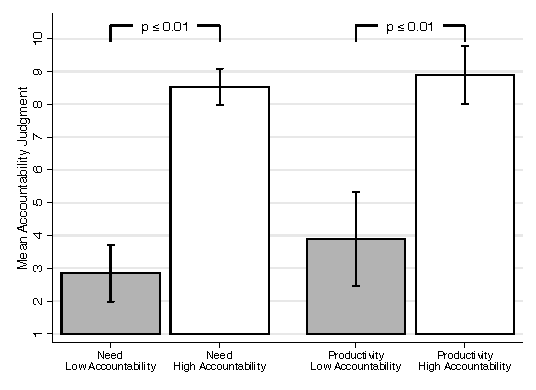
\includegraphics[scale=0.7]{figures/pilot_accountability.pdf}
   \begin{minipage}{10cm}
   \footnotesize
   \emph{The figure shows participants' mean judgments of Schneider's accountability for her greater need (lower productivity) in the low (high) accountability treatment using a $[1,10]$ scale. Larger numbers mean greater accountability. Bars represent $N=53$ ($N=29$) observations in the need (productivity) scenario. Error bars represent 90\% confidence intervals for the mean. $p$ value of a pairwise two-tailed t-test (within-participants treatment). Although the two different versions of the questionnaire were evenly distributed in a large classroom before students entered the it in order to attend a lecture, the case numbers of the pretest are not balanced due to group formation in the room.}
   \end{minipage}
   \caption{Pretest: Mean Accountability Judgment by Treatment and Scenario}
   \label{fig:pretest}
\end{figure}
%
\clearpage
%
\section{Regression Analysis}\label{sec:regression}
%
\subsection*{Details}
The marginal effects of scenario, supply situation, and accountability displayed in Figure \ref{fig:marginaleffect} are based on regression analyses. Table \ref{tab:regression_share} shows the results of a GLS random effects panel regression with robust standard errors on the \textit{share of logs} distributed to A as the endogenous variable. All models include scenario-order and case-order dummies that control for the randomization of the order in which the vignettes were presented to the participants. Model (1) provides an isolated test for scenario differences; model (2) tests for the isolated effect of high accountability; model (3) interacts scenario and accountability treatment; model (4) additionally includes the participants' socio-demographics and attitudes as covariates; model (5) includes case dummies and all possible interactions between scenario, treatment, and case; model (6) additionally includes the participants' socio-demographics and attitudes as covariates.\par
%
Since models (5) and (6) include 16 additional coefficients and interaction terms, we only report the main effects of scenario, accountability, and their interaction in the table (the full regression output is available from the authors on request). The marginal effects of scenario and accountability treatment (by case) estimated by the ``full'' model (6) are shown in the left panel of Tables \ref{tab:marginalscen} (Productivity Scenario) and \ref{tab:marginalaccount} (High Accountability Treatment). They are also displayed in the top and bottom left panels of Figure \ref{fig:marginaleffect}.\par
%
Analogously, Table \ref{tab:regression_dev} shows the results of a GLS random effects panel regression with robust standard errors on the \textit{deviation from the equal split} as the endogenous variable. Again, there are six different models where model (6) is the ``full'' model including all case dummies and interactions, control variables, and scenario-order as well as case-order dummies. The marginal effects of scenario and accountability treatment (by case) estimated by this model are shown in the right panel of Tables \ref{tab:marginalscen} (Productivity Scenario) and \ref{tab:marginalaccount} (High Accountability Treatment). They are also displayed in the top and bottom right panels of Figure \ref{fig:marginaleffect} in the main text.\par
%
Additionally, Table \ref{tab:symmetry} reports the results of the test on symmetry of the scenarios (\textbf{H3}). The effect of the supply situation on the share of logs and the deviation from the equal split (\textbf{H4}) is tested in Table \ref{tab:cases}. Table \ref{tab:regression_share_cov} shows the \textit{control variables} of regression models (4) and (6).\par
%
\subsection*{Regression Tables}
%
\newcommand{\rl}{\multicolumn{1}{c}{---}}
%
\begin{landscape}
\begin{table}[ht!]
\centering
\caption{Share of Logs Distributed to Person A: Regression Results}\label{tab:regression_share}
{\footnotesize
{
\def\sym#1{\ifmmode^{#1}\else\(^{#1}\)\fi}
\begin{tabularx}{16cm}{l*{6}{c}}\hline
                                 & \multicolumn{1}{c}{(1)}   & \multicolumn{1}{c}{(2)}   & \multicolumn{1}{c}{(3)}   & \multicolumn{1}{c}{(4)}   & \multicolumn{1}{c}{(5)}   &\multicolumn{1}{c}{(6)}   \\\hline\hline
   Scenario                      & $-0.132$\sym{***}         & \rl                       & $-0.120$\sym{***}         & $-0.120$\sym{***}         & $-0.0830$\sym{***}        &  $-0.0829$\sym{***}      \\
   $\{0=Need,1=Productivity\}$   &  (0.00773)                &                           &  (0.0122)                 &  (0.0122)                 &  (0.00968)                &   (0.00967)              \\
   [1em]
   Accountability                & \rl                       & $-0.0585$\sym{***}        & $-0.0473$\sym{***}        & $-0.0285$\sym{***}        & $-0.0123$                 &    0.00637               \\
   $\{0=low,1=high\}$            &                           &  (0.00908)                &  (0.00865)                &  (0.00872)                &  (0.00938)                &   (0.0102)               \\
   [1em]
   Accountability                & \rl                       & \rl                       & $-0.0224$                 & $-0.0231$                 & $-0.0212$\sym{*}          &  $-0.0219$\sym{*}        \\
   $\times$ Scenario             &                           &                           &  (0.0156)                 &  (0.0156)                 &  (0.0121)                 &   (0.0122)               \\
   [1em]
   Constant                      &   0.555\sym{***}          &   0.513\sym{***}          &   0.579\sym{***}          &   0.526\sym{***}          &   0.543\sym{***}          &    0.491\sym{***}        \\
                                 &  (0.00717)                &  (0.00931)                &  (0.00945)                &  (0.0345)                 &  (0.00859)                &   (0.0345)               \\\hline
   Case Dummies and              & No                        & No                        & No                        & No                        & Yes                       & Yes                      \\
   Interactions                  &                           &                           &                           &                           &                           &                          \\
   Control Variables             & No                        & No                        & No                        & Yes                       & No                        & Yes                      \\
   Scenario-Order and            & Yes                       & Yes                       & Yes                       & Yes                       & Yes                       & Yes                      \\
   Case-Order Dummies            &                           &                           &                           &                           &                           &                          \\\hline
   $\chi^2$                      & 328.8\sym{***}            &  56.51\sym{***}           & 357.9\sym{***}            & 731.7\sym{***}            & 740.4\sym{***}            & 1399.3\sym{***}          \\
   $R^2$ within                  &   0.358                   &   0.00185                 &   0.360                   &   0.361                   &   0.423                   &    0.423                 \\
   $R^2$ between                 &   0.00237                 &   0.178                   &   0.177                   &   0.551                   &   0.177                   &    0.551                 \\
   $R^2$ overall                 &   0.257                   &   0.0517                  &   0.308                   &   0.415                   &   0.353                   &    0.460                 \\\hline
\multicolumn{7}{p{15.5cm}}{\footnotesize \textit{The table reports the results of a GLS random effects panel regression with robust standard errors. Endogenous variable: Share of logs distributed to Person A ($\mbox{logshare}_A$). First row: coefficients, second row: standard errors in parentheses. Control variables include Age, Gender, Equivalent Household Net Income, Accountability Judgment, Smoker, Cardiovascular Disease, Metabolic Disease, Importance of Need, Importance of Equity, Importance of Equality, Locus of Control, Political Attitude (see Table \ref{tab:regression_share_cov} in the Appendix). $N=2000$ ($200$ participants). Significance levels: \sym{*} \(p<0.10\), \sym{**} \(p<0.05\), \sym{***} \(p<0.01\).}}
\end{tabularx}
}}
\end{table}
\end{landscape}
%
\clearpage
%
\begin{landscape}
\begin{table}[ht!]
\centering
\caption{Deviation from the Equal Split: Regression Results}\label{tab:regression_dev}
{\footnotesize
{
\def\sym#1{\ifmmode^{#1}\else\(^{#1}\)\fi}
\begin{tabularx}{16cm}{l*{6}{c}}\hline
                                 & \multicolumn{1}{c}{(1)}   & \multicolumn{1}{c}{(2)}   & \multicolumn{1}{c}{(3)}   & \multicolumn{1}{c}{(4)}   & \multicolumn{1}{c}{(5)}   & \multicolumn{1}{c}{(6)}   \\\hline\hline
   Scenario                      &  0.102\sym{**}            & \rl                       &   0.126\sym{**}           &   0.107\sym{**}           &   0.306\sym{***}          &   0.288\sym{***}          \\
   $\{0=Need,1=Productivity\}$   & (0.0467)                  &                           &  (0.0545)                 &  (0.0536)                 &  (0.0879)                 &  (0.0868)                 \\
   [1em]
   Accountability                & \rl                       & $-0.273$\sym{***}         & $-0.218$\sym{***}         & $-0.237$\sym{***}         & $-0.125$                  & $-0.145$                  \\
   N: $\{0=low,1=high\}$         &                           &  (0.0429)                 &  (0.0433)                 &  (0.0506)                 &  (0.0944)                 &  (0.0985)                 \\
   P: $\{0=high,1=low\}$                                                                                                                                                                                 \\
   [1em]
   Accountability                & \rl                       & \rl                       & $-0.0954$                 & $-0.0575$                 & $-0.198$\sym{*}           & $-0.161$                  \\
   $\times$ Scenario             &                           &                           &  (0.0711)                 &  (0.0742)                 &  (0.118)                  &  (0.120)                  \\
   [1em]
   Constant                      &  0.199\sym{***}           &   0.387\sym{***}          &  0.317\sym{***}           &   0.528\sym{***}          &   0.345\sym{***}          &   0.556\sym{***}          \\
                                 & (0.0376)                  &  (0.0405)                 & (0.0467)                  &  (0.148)                  &  (0.0771)                 &  (0.154)                  \\\hline
   Case Dummies and              & No                        & No                        & No                        & No                        & Yes                       & Yes                       \\
   Interactions                  &                           &                           &                           &                           &                           &                           \\
   Control Variables             & No                        & No                        & No                        & Yes                       & No                        & Yes                       \\
   Scenario-Order and            & Yes                       & Yes                       & Yes                       & Yes                       & Yes                       & Yes                       \\
   Case-Order Dummies            &                           &                           &                           &                           &                           &                           \\\hline
   $\chi^2$                      & 38.62\sym{***}            &  72.42\sym{***}           & 95.22\sym{***}            & 211.2\sym{***}            & 632.0\sym{***}            & 937.5\sym{***}            \\
   $R^2$ within                  &  0.0152                   &   0.0877                  &  0.0945                   &   0.0944                  &   0.170                   &   0.170                   \\
   $R^2$ between                 &  0.0564                   &   0.0567                  &  0.0654                   &   0.339                   &   0.0646                  &   0.339                   \\
   $R^2$ overall                 &  0.0246                   &   0.0806                  &  0.0878                   &   0.150                   &   0.146                   &   0.209                   \\\hline
\multicolumn{7}{p{15.5cm}}{\footnotesize \textit{The table reports the results of a GLS random effects panel regression. Endogenous variable: Deviation from the Equal Split ($\mbox{deviation}_A$). First row: coefficients, second row: standard errors in parentheses. Control variables include Age, Gender, Equivalent Household Net Income, Accountability Judgment, Smoker, Cardiovascular Disease, Metabolic Disease, Importance of Need, Importance of Equity, Importance of Equality, Locus of Control, Political Attitude (see Table \ref{tab:regression_share_cov} in the Appendix). All regressions include scenario- and case-order dummies. $N=2000$ ($200$ participants). Significance levels: \sym{*} \(p<0.10\), \sym{**} \(p<0.05\), \sym{***} \(p<0.01\).}}
\end{tabularx}
}}
\end{table}
\end{landscape}
%
\clearpage
%
\begin{table}[ht]
\centering
\caption{Control Variables}\label{tab:regression_share_cov}
{\footnotesize
{
\def\sym#1{\ifmmode^{#1}\else\(^{#1}\)\fi}
\begin{tabularx}{13.5cm}{lccccc}\hline
                            & \multicolumn{2}{c}{$\mbox{logshare}_A$}              &   & \multicolumn{2}{c}{$\mbox{deviation}_A$}              \\\cline{2-3}\cline{5-6}
                            & \multicolumn{1}{c}{(4)}   &\multicolumn{1}{c}{(6)}   &   & \multicolumn{1}{c}{(4)}   & \multicolumn{1}{c}{(6)}   \\\hline\hline
   Age                      &   0.000292               &   0.000290                &   & $-0.00146$                & $-0.00146$                \\
   $\{\sharp years\}$       &  (0.000244)              &  (0.000245)               &   &  (0.000937)               &  (0.000944)               \\
   [1em]
   Male                     & $-0.00506$               & $-0.00506$                &   & $-0.0248$                 & $-0.0248$                 \\
   $\{0=female,1=male\}$    &  (0.00708)               &  (0.00710)                &   &  (0.0317)                 &  (0.0319)                 \\
   [1em]
   Equiv. HH Net Income.    &   0.00000111\sym{***}    &   0.00000111\sym{***}     &   & $-0.00000853$\sym{**}     & $-0.00000856$\sym{**}     \\
   $\{euros\}$              &  (0.000000427)           &  (0.000000426)            &   &  (0.00000418)             &  (0.00000422)             \\
   [1em]
   Smoker                   &   0.0224\sym{**}         &   0.0224\sym{**}          &   & $-0.0725$\sym{*}          & $-0.0721$\sym{*}          \\
   $\{0=no,1=yes\}$         &  (0.00889)               &  (0.00893)                &   &  (0.0402)                 &  (0.0403)                 \\
   [1em]
   Cardiovascular Disease   &   0.00332                &   0.00327                 &   & $-0.0737$                 & $-0.0740$                 \\
   $\{0=no,1=yes\}$         &  (0.00940)               &  (0.00942)                &   &  (0.0489)                 &  (0.0490)                 \\
   [1em]
   Metabolic Disease=1      &   0.00508                &   0.00515                 &   &   0.0559                  &   0.0566                  \\
   $\{0=no,1=yes\}$         &  (0.0117)                &  (0.0117)                 &   &  (0.0502)                 &  (0.0504)                 \\
   [1em]
   Locus of Control         &   0.000553               &   0.000554                &   &   0.00590                 &   0.00585                 \\
   $\{1,\ldots,7\}$         &  (0.00319)               &  (0.00320)                &   &  (0.0180)                 &  (0.0181)                 \\
   [1em]
   Political Attitude       & $-0.00464$               & $-0.00462$                &   &   0.0300\sym{**}          &   0.0300\sym{**}          \\
   $\{1,\ldots,7\}$         &  (0.00314)               &  (0.00315)                &   &  (0.0132)                 &  (0.0133)                 \\
   [1em]
   Importance Need          &   0.00965\sym{***}       &   0.00964\sym{***}        &   &   0.00801                 &   0.00805                 \\
   $\{1,\ldots,7\}$         &  (0.00207)               &  (0.00208)                &   &  (0.00995)                &  (0.00998)                \\
   [1em]
   Importance Equity        & $-0.0130$\sym{***}       & $-0.0130$\sym{***}        &   & $-0.00122$                & $-0.00126$                \\
   $\{1,\ldots,7\}$         &  (0.00240)               &  (0.00241)                &   &  (0.0118)                 &  (0.0119)                 \\
   [1em]
   Importance Equality      &   0.00913\sym{***}       &   0.00913\sym{***}        &   & $-0.0618$\sym{***}        & $-0.0619$\sym{***}        \\
   $\{1,\ldots,7\}$         &  (0.00211)               &  (0.00211)                &   &  (0.00953)                &  (0.00959)                \\
   [1em]
   Acc. Judgment            &   0.00306                &   0.00312                 &   & $-0.00525$                & $-0.00522$                \\
   $\{1,\ldots,7\}$         &  (0.00229)               &  (0.00234)                &   &  (0.0109)                 &  (0.0111)                 \\
   [1em]\hline
\multicolumn{6}{p{13cm}}{\footnotesize \textit{The table reports the results of a GLS random effects panel regressions with robust standard errors (control variables of models (4) and (6) in Table \ref{tab:regression_share} and in Table \ref{tab:regression_dev}). First row: coefficients, second row: standard errors in parentheses. Significance levels: \sym{*} \(p<0.10\), \sym{**} \(p<0.05\), \sym{***} \(p<0.01\).}}
\end{tabularx}
}}
\end{table}
%
\clearpage
%
\begin{table}[ht]
\centering
\caption{Marginal Effect of the Productivity Scenario}\label{tab:marginalscen}
{\footnotesize
\def\sym#1{\ifmmode^{#1}\else\(^{#1}\)\fi}
\begin{tabular}{cccccccc}\\[0.5ex]\hline
                            & \multicolumn{3}{c}{$\Delta\mbox{logshare}_A$}                                             &   & \multicolumn{3}{c}{$\Delta\mbox{deviation}_A$}                                            \\\cline{2-4}\cline{6-8}
   \multicolumn{1}{c}{Case} & \multicolumn{1}{c}{Low}   & \multicolumn{1}{c}{High}   & \multicolumn{1}{c}{Difference}   &   & \multicolumn{1}{c}{Low}   & \multicolumn{1}{c}{High}   & \multicolumn{1}{c}{Difference}   \\\hline\hline
   1                        & $-0.083$\sym{***}         & $-0.105$\sym{***}          & $-0.022$\sym{*}                  &   &   0.288\sym{***}          &   0.127                    &   0.161                          \\
                            &  (0.010)                  &  (0.007)                   &  (0.012)                         &   &  (0.087)                  &  (0.100)                   &  (0.120)                         \\
   2                        & $-0.106$\sym{***}         & $-0.115$\sym{***}          & $-0.010$                         &   & $-0.272$\sym{***}         & $-0.284$\sym{***}          & $-0.012$                         \\
                            &  (0.010)                  &  (0.009)                   &  (0.014)                         &   &  (0.066)                  &  (0.078)                   &  (0.101)                         \\
   3                        & $-0.115$\sym{***}         & $-0.139$\sym{***}          & $-0.024$                         &   &   0.113\sym{*}            &   0.052                    & $-0.061$                         \\
                            &  (0.016)                  &  (0.010)                   &  (0.019)                         &   &  (0.064)                  &  (0.067)                   &  (0.085)                         \\
   4                        & $-0.132$\sym{***}         & $-0.153$\sym{***}          & $-0.021$                         &   &   0.176\sym{**}           &   0.171\sym{***}           & $-0.005$                         \\
                            &  (0.018)                  &  (0.016)                   &  (0.024)                         &   &  (0.070)                  &  (0.061)                   &  (0.088)                         \\
   5                        & $-0.163$\sym{***}         & $-0.201$\sym{***}          & $-0.038$                         &   &   0.231\sym{***}          &   0.182\sym{***}           & $-0.049$                         \\
                            &  (0.020)                  &  (0.018)                   &  (0.028)                         &   &  (0.062)                  &  (0.058)                   &  (0.079)                         \\\hline
   All                      & $-0.120$\sym{***}         & $-0.143$\sym{***}          & $-0.023$                         &   &   0.107\sym{**}           &   0.050                    &   0.057                          \\
                            &  (0.012)                  &  (0.010)                   &  (0.016)                         &   &  (0.054)                  &  (0.061)                   &  (0.075)                         \\\hline
\multicolumn{8}{p{12cm}}{\footnotesize{\textit{The table reports the marginal effect of the Productivity Scenario on the share of logs distributed to Person A ($\Delta\mbox{logshare}_A$) and the deviation from the equal split ($\Delta\mbox{deviation}_A$). GLS effects panel model estimates are reported in Table \ref{tab:regression_share} (share of logs) and in Table \ref{tab:regression_dev} (deviation). $N=2000$. First row: coefficients, second row: standard errors in parentheses. Significance levels: \sym{*} \(p<0.10\), \sym{**} \(p<0.05\), \sym{***} \(p<0.01\).}}}
\end{tabular}
}
\end{table}
%
\clearpage
%
\begin{table}[ht]
\centering
\caption{Symmetry of the Scenarios}\label{tab:symmetry}
{\footnotesize
\def\sym#1{\ifmmode^{#1}\else\(^{#1}\)\fi}
\begin{tabular}{cccccccc}\\[0.5ex]\hline
         & \multicolumn{3}{c}{Low Accountability}    &   & \multicolumn{3}{c}{High Accountability}   \\\cline{2-4}\cline{6-8}
   Case  & Need      & Productivity   & $p$          &   & Need      & Productivity & $p$            \\\hline\hline
   1     &  0.532    &  0.450         & 0.105        &   &  0.539    &  0.434    & 0.004             \\
         & (0.008)   & (0.007)        & ($=$)        &   & (0.007)   & (0.005)   & (P)               \\
   2     &  0.581    &  0.476         & 0.000        &   &  0.565    &  0.450    & 0.117             \\
         & (0.007)   & (0.008)        & (N)          &   & (0.007)   & (0.005)   & ($=$)             \\
   3     &  0.575    &  0.460         & 0.017        &   &  0.533    &  0.394    & 0.000             \\
         & (0.010)   & (0.012)        & (N)          &   & (0.007)   & (0.008)   & (P)               \\
   4     &  0.563    &  0.431         & 0.728        &   &  0.531    &  0.378    & 0.000             \\
         & (0.011)   & (0.014)        & ($=$)        &   & (0.007)   & (0.014)   & (P)               \\
   5     &  0.584    &  0.421         & 0.812        &   &  0.524    &  0.324    & 0.000             \\
         & (0.013)   & (0.017)        & ($=$)        &   & (0.007)   & (0.015)   & (P)               \\\hline
   All   &  0.567    &  0.447         & 0.219        &   &  0.538    &  0.396    & 0.000             \\
         & (0.007)   & (0.010)        & ($=$)        &   & (0.005)   & (0.007)   & (P)               \\\hline
\multicolumn{8}{p{12cm}}{\footnotesize{\textit{The table reports the share of logs distributed to Person A ($\Delta\mbox{logshare}_A^s$) by scenario and accountability treatment estimated by a GLS random effects panel model (marginal effects). Estimates are reported in Table \ref{tab:regression_share}. First row: coefficients, second row: standard errors in parentheses. $p$ gives the significance level of testing symmetry of the scenarios (H3): $\Delta\mbox{logshare}_A^N=1-\Delta\mbox{logshare}_A^s$. Here, $=$ means that the null hypothesis of symmetry cannot be rejected; N (P) means that the equality sign has to be replaced by $>$ ($<$).}}}
\end{tabular}
}
\end{table}
%
\clearpage
%
\begin{table}[ht]
\centering
\caption{Marginal Effect of High Accountability}\label{tab:marginalaccount}
{\footnotesize
\def\sym#1{\ifmmode^{#1}\else\(^{#1}\)\fi}
\begin{tabular}{cccccccc}\\[0.5ex]\hline
                               & \multicolumn{3}{c}{$\Delta\mbox{logshare}_A$}                                                    &   & \multicolumn{3}{c}{$-1\times|\Delta\mbox{deviation}_A|$}                                         \\\cline{2-4}\cline{6-8}
   \multicolumn{1}{c}{Case}    & \multicolumn{1}{c}{Need}   & \multicolumn{1}{c}{Productivity} & \multicolumn{1}{c}{Difference}   &   & \multicolumn{1}{c}{Need} & \multicolumn{1}{c}{Productivity}   & \multicolumn{1}{c}{Difference}   \\\hline\hline
   1                           &  $0.006$                   & $-0.016$\sym{*}                  & $-0.022$\sym{*}                  &   & $-0.145$                 & $-0.305$\sym{***}                  & $-0.161$                         \\
                               &  (0.010)                   &  (0.009)                         &  (0.012)                         &   &  (0.098)                 &  (0.089)                           &  (0.120)                         \\
   2                           & $-0.016$                   & $-0.026$\sym{***}                & $-0.010$                         &   & $-0.275$\sym{***}        & $-0.287$\sym{*}                    & $-0.012$                         \\
                               &  (0.010)                   &  (0.010)                         &  (0.014)                         &   &  (0.074)                 &  (0.071)                           &  (0.101)                         \\
   3                           & $-0.042$\sym{***}          & $-0.066$\sym{***}                & $-0.024$                         &   & $-0.306$\sym{***}        & $-0.367$\sym{***}                  & $-0.061$                         \\
                               &  (0.012)                   &  (0.014)                         &  (0.019)                         &   &  (0.058)                 &  (0.072)                           &  (0.085)                         \\
   4                           & $-0.032$\sym{**}           & $-0.053$\sym{***}                & $-0.021$                         &   & $-0.216$\sym{***}        & $-0.220$\sym{***}                  & $-0.005$                         \\
                               &  (0.013)                   &  (0.020)                         &  (0.024)                         &   &  (0.055)                 &  (0.075)                           &  (0.088)                         \\
   5                           & $-0.059$\sym{***}          & $-0.097$\sym{***}                & $-0.038$                         &   & $-0.246$\sym{***}        & $-0.295$\sym{***}                  & $-0.049$                         \\
                               &  (0.015)                   &  (0.023)                         &  (0.028)                         &   &  (0.050)                 &  (0.068)                           &  (0.079)                         \\\hline
   All                         & $-0.029$\sym{***}          & $-0.052$\sym{***}                & $-0.023$                         &   & $-0.238$\sym{***}        & $-0.295$\sym{***}                  & $-0.057$                         \\
                               &  (0.009)                   &  (0.013)                         &  (0.016)                         &   &  (0.051)                 &  (0.064)                           &  (0.075)                         \\\hline
\multicolumn{8}{p{12cm}}{\footnotesize{\textit{The table reports the marginal effects of high accountability on the share of logs distributed to Person A ($\Delta\mbox{logshare}_A$) and the deviation from the equal split ($-1\times|\Delta\mbox{deviation}_A|$). GLS effects panel model estimates are reported in Table \ref{tab:regression_share} (share of logs) and in Table \ref{tab:regression_dev} (deviation). $N=2000$. First row: coefficients, second row: standard errors in parentheses. Significance levels: \sym{*} \(p<0.10\), \sym{**} \(p<0.05\), \sym{***} \(p<0.01\).}}}
\end{tabular}
}
\end{table}
%
\clearpage
%
\begin{table}[ht]
\centering
\caption{Case Differences}\label{tab:marginalcase}
{\footnotesize
\def\sym#1{\ifmmode^{#1}\else\(^{#1}\)\fi}
\begin{tabular}{cccccccccc}\\[0.5ex]\hline
\multicolumn{10}{c}{Share of Logs Distributed to A}                                                                           \\\hline
          & \multicolumn{9}{c}{Marginal Effect of Productivity Scenario}                                                      \\\cline{2-10}
          & \multicolumn{4}{c}{Low Accountability}                &   & \multicolumn{4}{c}{High Accountability}               \\\cline{2-5}\cline{7-10}
   Case   & 2           & 3           & 4           & 5           &   & 2           & 3           & 4           & 5           \\\hline
   1      & ns          & ns          & \sym{**}    & \sym{***}   &   & ns          & \sym{**}    & \sym{**}    & \sym{***}   \\
   2      & \rl         & ns          & ns          & ns          &   & \rl         & ns          & ns          & \sym{***}   \\
   3      & \rl         & \rl         & ns          & \sym{**}    &   & \rl         & \rl         & ns          & \sym{***}   \\
   4      & \rl         & \rl         & \rl         & ns          &   & \rl         & \rl         & \rl         & \sym{***}   \\\hline
          & \multicolumn{9}{c}{Marginal Effect of High Accountability}                                                        \\\cline{2-10}
          & \multicolumn{4}{c}{Need Scenario}                     &   & \multicolumn{4}{c}{Productivity Scenario}             \\\cline{2-5}\cline{7-10}
   Case   & 2           & 3           & 4           & 5           &   & 2           & 3           & 4           & 5           \\\hline
   1      & ns          & \sym{***}   & \sym{**}    & \sym{***}   &   & ns          & \sym{***}   & ns          & \sym{***}   \\
   2      & \rl         & ns          & ns          & \sym{**}    &   & \rl         & \sym{**}    & ns          & \sym{***}   \\
   3      & \rl         & \rl         & ns          & ns          &   & \rl         & \rl         & ns          & \sym{***}   \\
   4      & \rl         & \rl         & \rl         & ns          &   & \rl         & \rl         & \rl         & \sym{***}   \\\hline\hline
   \multicolumn{10}{c}{Deviation from the Equal Split}                                                                        \\\hline
          & \multicolumn{9}{c}{Marginal Effect of Productivity Scenario}                                                      \\\cline{2-10}
          & \multicolumn{4}{c}{Low Accountability}                &   & \multicolumn{4}{c}{High Accountability}               \\\cline{2-5}\cline{7-10}
   Case   & 2           & 3           & 4           & 5           &   & 2           & 3           & 4           & 5           \\\hline
   1      & \sym{***}   & ns          & ns          & ns          &   & \sym{***}   & ns          & ns          & ns          \\
   2      & \rl         & \sym{***}   & \sym{***}   & \sym{***}   &   & \rl         & \sym{***}   & \sym{***}   & \sym{***}   \\
   3      & \rl         & \rl         & ns          & ns          &   & \rl         & \rl         & \sym{**}    & \sym{**}    \\
   4      & \rl         & \rl         & \rl         & ns          &   & \rl         & \rl         & \rl         & ns          \\\hline
          & \multicolumn{9}{c}{Marginal Effect of High Accountability}                                                        \\\cline{2-10}
          & \multicolumn{4}{c}{Need Scenario}                     &   & \multicolumn{4}{c}{Productivity Scenario}             \\\cline{2-5}\cline{7-10}
   Case   & 2           & 3           & 4           & 5           &   & 2           & 3           & 4           & 5           \\\hline
   1      & ns          & ns          & ns          & ns          &   & ns          & ns          & ns          & ns          \\
   2      & \rl         & ns          & ns          & ns          &   & \rl         & ns          & ns          & ns          \\
   3      & \rl         & \rl         & ns          & ns          &   & \rl         & \rl         & \sym{**}    & ns          \\
   4      & \rl         & \rl         & \rl         & ns          &   & \rl         & \rl         & \rl         & ns          \\\hline
\multicolumn{10}{p{8cm}}{\footnotesize{\textit{The table shows pairwise comparisons of the marginal effects of the Productivity Scenario (High Accountability Treatment) on the logs distributed to A (deviation from the equal split). $ns=$not significant. Significance levels: \sym{*} \(p<0.10\), \sym{**} \(p<0.05\), \sym{***} \(p<0.01\). Bonferroni correction for multiple hypotheses testing.}}}
\end{tabular}
}
\end{table}
%
\section{Additional Tables}\label{sec:app_tables}
%
\begin{table}[ht]
   \centering
   \caption{Breakdown of Sample by Gender, Age, and Income}\label{tab:quota_demos}
   \begin{tabular}{rrrrrr}\\[0.5ex]\hline
   \multicolumn{2}{c}{Gender}   & \multicolumn{2}{c}{Age}   & \multicolumn{2}{c}{Income Interval$^a$}   \\\hline
   Group    & Share             & Group    & Share          & Group              & Share                \\\hline\hline
   Female   & 49.5              & 18--29   & 20.5           & [0, 1100)          & 20.0                 \\
   Male     & 50.5              & 30--39   & 18.5           & [1100, 1500)       & 20.0                 \\
            &                   & 40--49   & 19.0           & [1500, 2000)       & 20.0                 \\
            &                   & 50--59   & 24.0           & [2000, 2600)       & 20.0                 \\
            &                   & 60--69   & 18.0           & [2600, $\infty$)   & 20.0                 \\\hline
   \multicolumn{6}{p{8cm}}{\footnotesize{\textit{Share in percent. $N=200$. $^a$Equivalent household net income.}}}
   \end{tabular}
\end{table}
%
\clearpage
%
\begin{table}
\centering
\caption{Share of Logs Distributed to A: Means}\label{tab:share_means}
{\footnotesize
\def\sym#1{\ifmmode^{#1}\else\(^{#1}\)\fi}
\begin{tabularx}{13.5cm}{cccccccccc}\hline
          & \multicolumn{3}{c}{Low Accountability}              &   & \multicolumn{3}{c}{High Accountability}            &   & $\Delta$Low       \\\cline{2-4}\cline{6-8}
   Case   & $logshare_A$   & $p_A/p$        & $n_A/n$           &   & $logshare_A$   & $p_A/p$         & $n_A/n$         &   & High              \\\hline\hline
   \multicolumn{10}{c}{Need Scenario}                                                                                                            \\
   1      &   0.542        & 0.5\sym{***}   &  0.6\sym{***}     &   &  0.531         &  0.5\sym{***}   & 0.6\sym{***}    &   &  0.011            \\
          & (0.007)        & (.)            &  (.)              &   & (0.006)        &  (.)            & (.)             &   & (0.009)           \\
   2      &  0.591         & 0.5\sym{***}   &  0.64\sym{***}    &   &  0.557         &  0.5\sym{***}   & 0.64\sym{***}   &   &  0.034\sym{***}   \\
          & (0.007)        & (.)            &  (.)              &   & (0.007)        &  (.)            & (.)             &   & (0.010)           \\
   3      &  0.584         & 0.5\sym{***}   &  0.71\sym{***}    &   &  0.525         &  0.5\sym{***}   & 0.71\sym{***}   &   &  0.059\sym{***}   \\
          & (0.010)        & (.)            &  (.)              &   & (0.006)        &  (.)            & (.)             &   & (0.012)           \\
   4      &  0.572         & 0.5\sym{***}   &  0.78\sym{***}    &   &  0.522         &  0.5\sym{***}   & 0.78\sym{***}   &   &  0.050\sym{***}   \\
          & (0.012)        & (.)            &  (.)              &   & (0.006)        &  (.)            & (.)             &   & (0.013)           \\
   5      &  0.594         & 0.5\sym{***}   &  0.86\sym{***}    &   &  0.516         &  0.5\sym{**}    & 0.86\sym{***}   &   &  0.078\sym{***}   \\
          & (0.014)        & (.)            &  (.)              &   & (0.006)        &  (.)            & (.)             &   & (0.015)           \\\hline
   All    &  0.577         & 0.5\sym{***}   &  0.717\sym{***}   &   &  0.530         &  0.5\sym{***}   & 0.717\sym{***}  &   &  0.047\sym{***}   \\
          & (0.005)        & (.)            & (0.004)           &   & (0.003)        &  (.)            & (0.004)         &   & (0.006)           \\\hline\hline
   \multicolumn{10}{c}{Productivity Scenario}                                                                                                    \\
   1      &  0.459         & 0.4\sym{***}   &  0.5\sym{***}     &   &  0.426         &  0.4\sym{***}   & 0.5\sym{***}    &   &  0.033\sym{***}   \\
          & (0.008)        & (.)            &  (.)              &   & (0.005)        &  (.)            & (.)             &   & (0.009)           \\
   2      &  0.486         & 0.36\sym{***}  &  0.5\sym{**}      &   &  0.443         &  0.36\sym{***}  & 0.5\sym{***}    &   &  0.043\sym{***}   \\
          & (0.008)        & (.)            &  (.)              &   & (0.006)        &  (.)            & (.)             &   & (0.010)           \\
   3      &  0.469         & 0.29\sym{***}  &  0.5\sym{***}     &   &  0.386         &  0.29\sym{***}  & 0.5\sym{***}    &   &  0.083\sym{***}   \\
          & (0.013)        & (.)            &  (.)              &   & (0.010)        &  (.)            & (.)             &   & (0.016)           \\
   4      &  0.440         & 0.22\sym{***}  &  0.5\sym{***}     &   &  0.370         &  0.22\sym{***}  & 0.5\sym{***}    &   &  0.071\sym{***}   \\
          & (0.015)        & (.)            &  (.)              &   & (0.016)        &  (.)            & (.)             &   & (0.022)           \\
   5      &  0.431         & 0.14\sym{***}  &  0.5\sym{***}     &   &  0.316         &  0.14\sym{***}  & 0.5\sym{***}    &   &  0.115\sym{***}   \\
          & (0.018)        & (.)            &  (.)              &   & (0.018)        &  (.)            & (.)             &   & (0.025)           \\\hline
   All    &  0.457         & 0.283\sym{***} &  0.5\sym{***}     &   &  0.388         &  0.283\sym{***} & 0.5\sym{***}    &   &  0.069\sym{***}   \\
          & (0.006)        & (0.004)        &  (.)              &   & (0.006)        & (0.004)         & (.)             &   & (0.008)           \\\hline
\multicolumn{10}{p{13cm}}{\footnotesize\textit{Mean of $\mbox{logshare}_A$ by accountability treatment and scenario. First row: means; second row: standard errors in parentheses.  $p_A/p$: A's productivity share. $n_A/n$: A's need share. Asterisks denote the significance level of a one-tailed t-test: $p(\mbox{logshare}_A>p_A/p)$, $p(\mbox{logshare}_A<n_A/n)$, and $p(\mbox{logshare}_A^{\mbox{low}}-\mbox{logshare}_A^{\mbox{high}}>0)$. Low (High) Accountability Treatment: $N=91$ $(109)$ observations per case; $N=455$ $(545)$ observations in total per scenario. Significance levels: \sym{*} \(p<0.10\), \sym{**} \(p<0.05\), \sym{***} \(p<0.01\).}}
\end{tabularx}
}
\end{table}
%
\clearpage
%
\begin{table}
\centering
\caption{Deviation from the Equal Split: Means}\label{tab:dev_means}
{\footnotesize
\def\sym#1{\ifmmode^{#1}\else\(^{#1}\)\fi}
\begin{tabularx}{12.5cm}{cccccccccc}\hline
             &\multicolumn{4}{c}{Need Scenario}                 &   & \multicolumn{4}{c}{Productivity Scenario}          \\\cline{2-5}\cline{7-10}
   Case      & Low Acc.   & High Acc.   &   & $\Delta$          &   & Low Acc.   & High Acc.   &   & $\Delta$            \\\hline\hline
   1         &  0.423     &  0.309      &   &  0.114            &   &  0.410     &  0.745      &   & $-0.334$\sym{***}   \\
             & (0.072)    & (0.062)     &   & (0.095)           &   & (0.077)    & (0.051)     &   & (0.092)             \\
   2         &  0.671     &  0.419      &   &  0.252\sym{***}   &   &  0.106     &  0.420      &   & $-0.314$\sym{***}   \\
             & (0.049)    & (0.051)     &   & (0.070)           &   & (0.055)    & (0.045)     &   & (0.071)             \\
   3         &  0.392     &  0.116      &   &  0.276\sym{***}   &   &  0.143     &  0.532      &   & $-0.389$\sym{***}   \\
             & (0.047)    & (0.029)     &   & (0.055)           &   & (0.060)    & (0.047)     &   & (0.076)             \\
   4         &  0.260     &  0.080      &   &  0.180\sym{***}   &   &  0.214     &  0.469      &   & $-0.254$\sym{**}    \\
             & (0.042)    & (0.022)     &   & (0.047)           &   & (0.055)    & (0.057)     &   & (0.079)             \\
   5         &  0.262     &  0.045      &   &  0.217\sym{***}   &   &  0.193     &  0.514      &   & $-0.321$\sym{***}   \\
             & (0.039)    & (0.018)     &   & (0.043)           &   & (0.052)    & (0.049)     &   & (0.071)             \\
   All       &  0.402     &  0.194      &   &  0.208\sym{***}   &   &  0.213     &  0.536      &   & $-0.323$\sym{***}   \\
             & (0.024)    & (0.019)     &   & (0.030)           &   & (0.027)    & (0.023)     &   & (0.035)             \\\hline
\multicolumn{10}{p{12.25cm}}{\footnotesize\textit{Mean of $\mbox{deviation}_A$ by accountability treatment and scenario. First row: means; second row: standard errors in parentheses. $N=91$ ($109$) per case in low (high) accountability; total cases: $N=455$ ($545$). Asterisks denote the significance level of a one-tailed t-test. Significance levels: \sym{*} \(p<0.10\), \sym{**} \(p<0.05\), \sym{***} \(p<0.01\).}}
\end{tabularx}
}
\end{table}
%
\end{document}
